\documentclass[12pt]{article}
\usepackage{amssymb, amsmath, amsfonts, bm, graphicx, geometry,cancel}
\usepackage{tabularx, booktabs, float, enumitem, multicol, mathtools}
\geometry{margin=1in}


\title{}
\date{}
\author{}

\begin{document}
{\centering\LARGE PH-214 Modern Physics Notes\par}
\section*{Useful Math}
\textbf{Taylor series expansions:}
\begin{flalign*}
\sin x &= \sum_{n=0}^{\infty} (-1)^n \frac{x^{2n+1}}{(2n+1)!} 
       = x - \frac{x^3}{3!} + \frac{x^5}{5!} - \frac{x^7}{7!} + \cdots & \\[6pt]
\cos x &= \sum_{n=0}^{\infty} (-1)^n \frac{x^{2n}}{(2n)!} 
       = 1 - \frac{x^2}{2!} + \frac{x^4}{4!} - \frac{x^6}{6!} + \cdots & \\[6pt]
\tan x &= \sum_{n=1}^{\infty} \frac{B_{2n} (-4)^n (1-4^n)}{(2n)!}\,x^{2n-1} 
       = x + \frac{x^3}{3} + \frac{2x^5}{15} + \frac{17x^7}{315} + \cdots & \\[6pt]
(1+x)^m &= \sum_{n=0}^{\infty} \binom{m}{n} x^n 
       = 1 + mx + \frac{m(m-1)}{2}x^2 + \frac{m(m-1)(m-2)}{6}x^3 + \cdots &
\end{flalign*}
\underline{Note:} For small x, higher order terms reduce to zero\\\\
\textbf{Euler's Identity:}\\ Use complex exponentials to manipulate complicated trig functions and complex amplitudes.
\[e^{ix} = \cos x + i \sin x\]
\textbf{Visualizing propagating plane waves:}\\
A 1D plane wave propagating in the $+z$ direction can be mathematically represented as:
\[\psi = f(kz - \omega t)\]
Where:
\begin{itemize}[label=\textopenbullet]
       \item $(kz - \omega t)$ [rad]:\\ The argument represents the \textbf{phase} of the wave. A change in phase simply moves the wave forward or backward in space and time, without changing its shape, there are a few ways to see this which we will look at later.
       \item $k$ [rad/m]:\\ is the \textbf{wave number}, representing the spatial frequency of the wave, or how \textit{spread out} the wave is in space. Since $k$ scales the spatial variable $z$, a larger $k$ means the wave advances through the same phase over a smaller change in $z$.
       \item $\omega$ [rad/s]:\\ is the \textbf{angular frequency}, representing the temporal frequency of the wave, or how \textit{spread out} the wave is in time. As in rotational kinematics, $\omega$ scales time $t$, and a larger $\omega$ means the wave advances through the same phase over a smaller change in $t$.
\end{itemize}
A plane wave is special in that it represents a wave whose shape is fixed as it propagates through space and time, with it’s shape represented by the function $f$.\\\\
\underline{Note:}
\[\boxed{k=\frac{2\pi}{\lambda},\quad \frac{\omega}{2\pi} = f = \frac{1}{T}\,[\text{Hz}],\quad v=\frac{\omega}{k}}\]
\textbf{Global View}\\
As mentioned before, there are two ways to visualize how the phase $(kz - \omega t)$ represents a propagating wave. The first is a \textit{global} view, looking at how $z$ and $t$ change relative to each other for a fixed phase, tracking a specific point on the wave.
\begin{center}
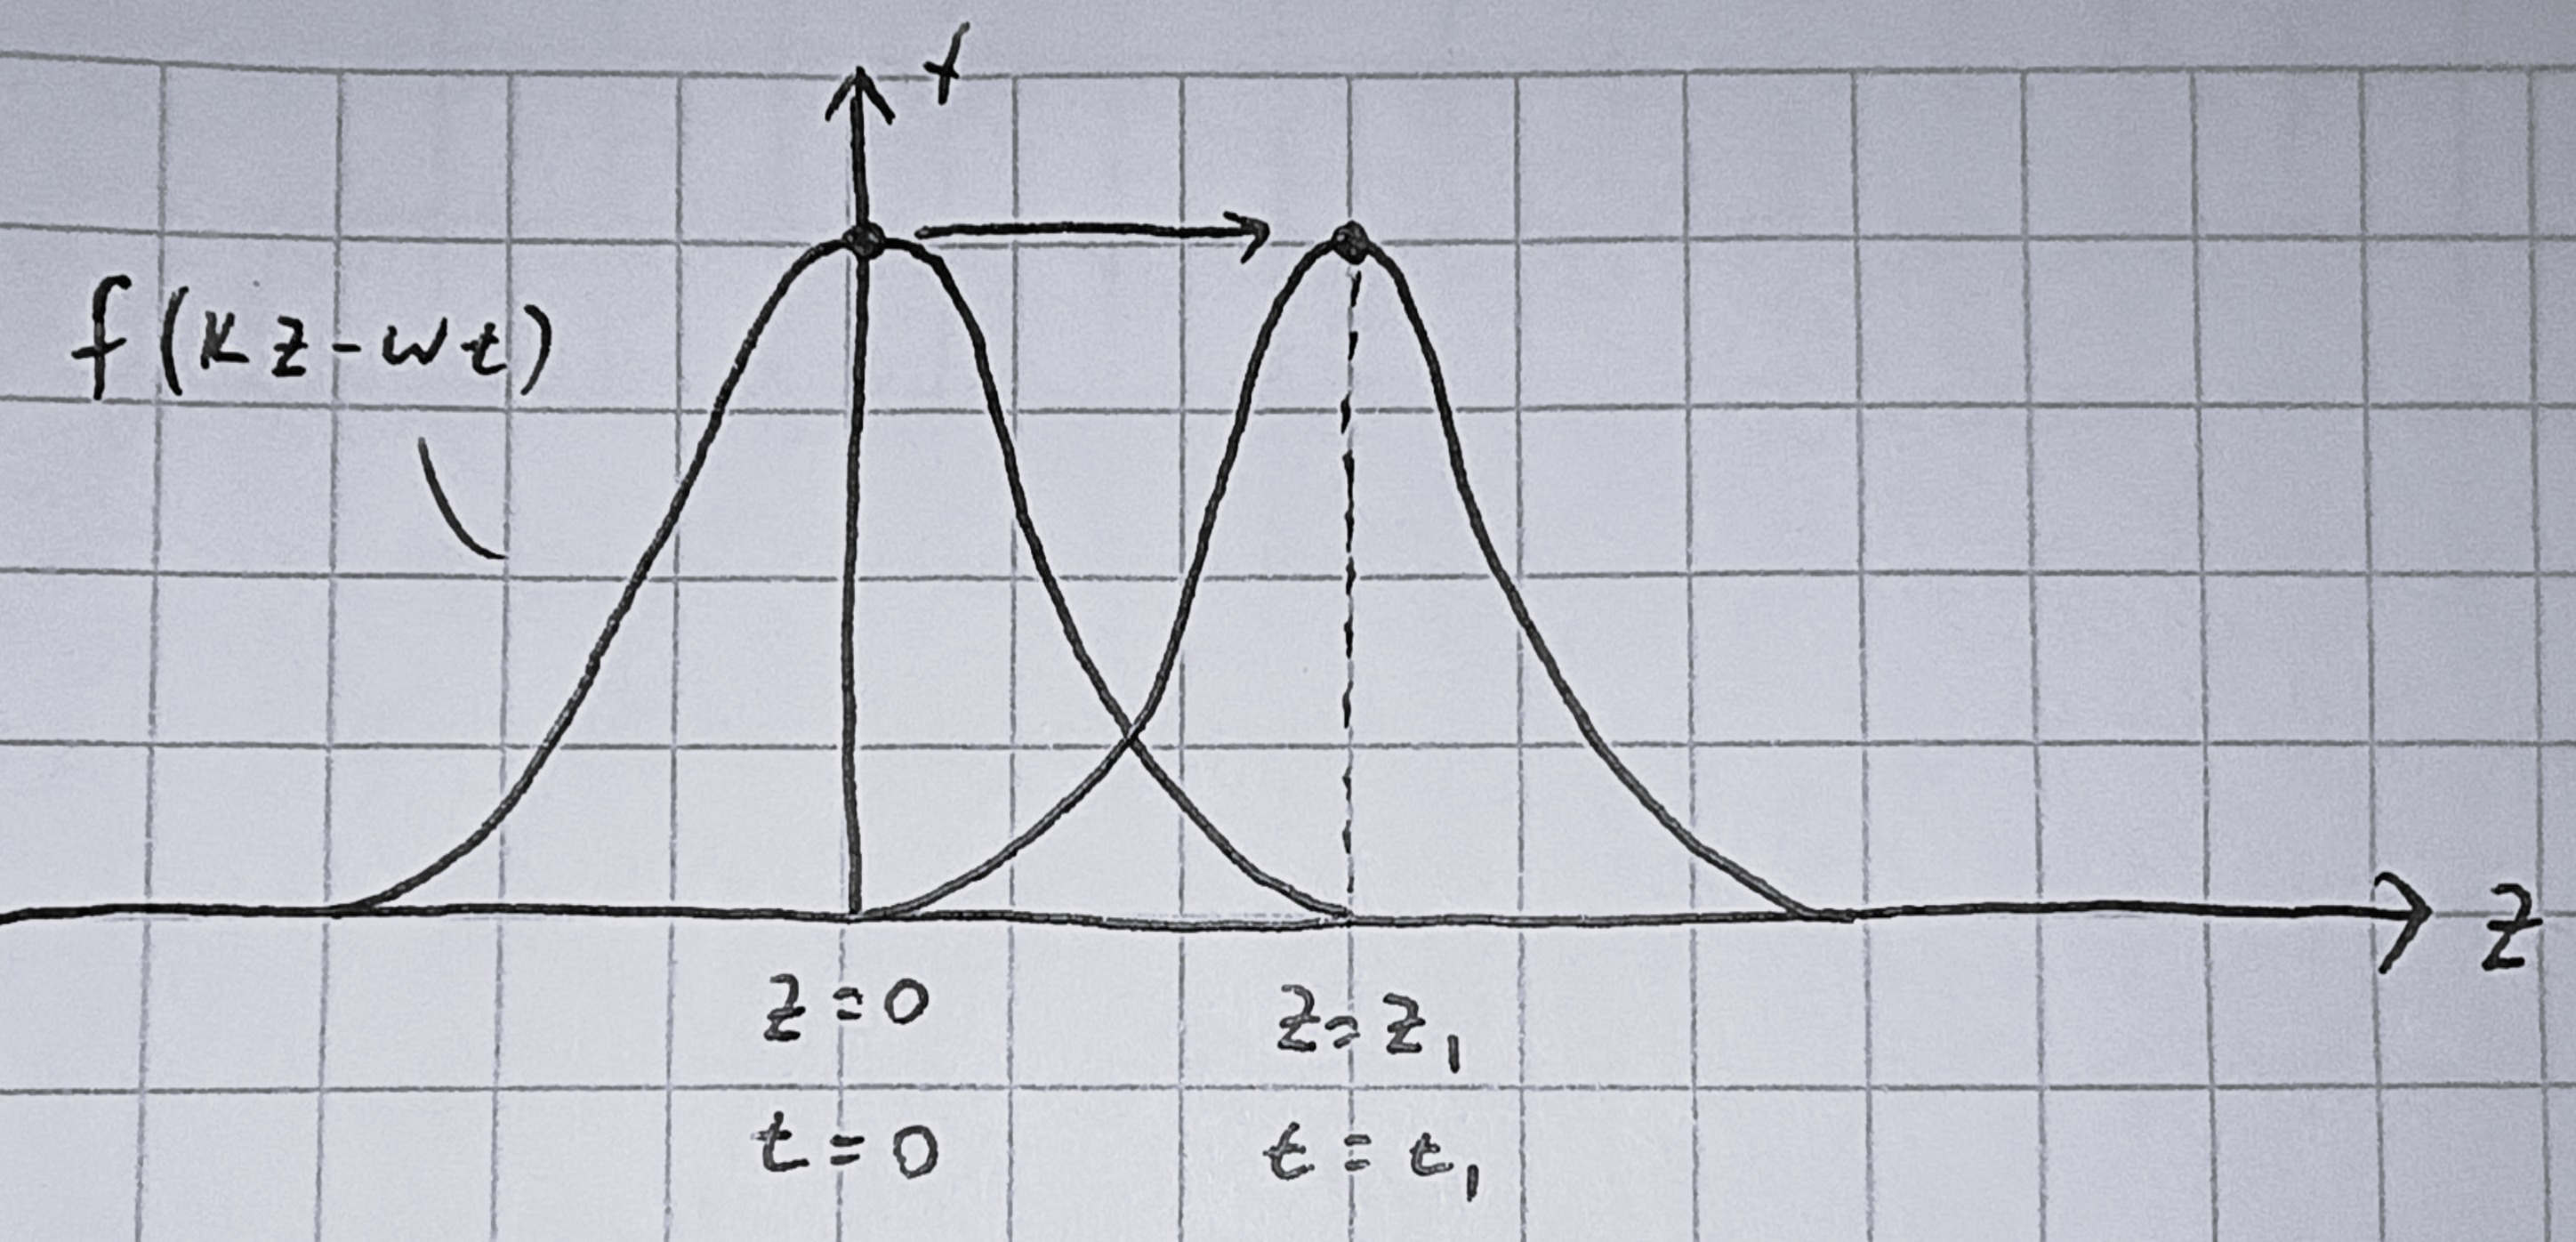
\includegraphics[width=0.5\textwidth]{1d Plane Wave.jpg}
\end{center}
When we track a specific point on the wave, $f$ must give the same value at different positions and times, meaning the phase must stay constant. This shows that as $t$ increases, $z$ must also increase to maintain the phase (the wave moves rightward!). Vice versa, as $z$ increases, $t$ must increase too to keep the phase constant (again, moving rightward!).\\\\
\underline{Note:} This intuition applies to \textit{any} point on the wave! Thus, by tracking all points, we can clearly see a propagating plane wave.\\\\
\textbf{Local View}\\
The second is a \textit{local} view, looking at how the phase changes at a fixed position as time changes, or at a fixed time as position changes. For this, we will look at a sinusoidal wave, to better show oscillation: $\psi = cos(kz - \omega t)$
\begin{enumerate}
       \item Fixing $z$, letting $t$ vary:\\
       Imagine we are at a fixed position $z=z_1$. As time increases, we are effectively watching a cross-section of the wave at that point, seeing only a single point along the wave moving up and down like riding the “surface” of the wave. 
       \begin{center}
       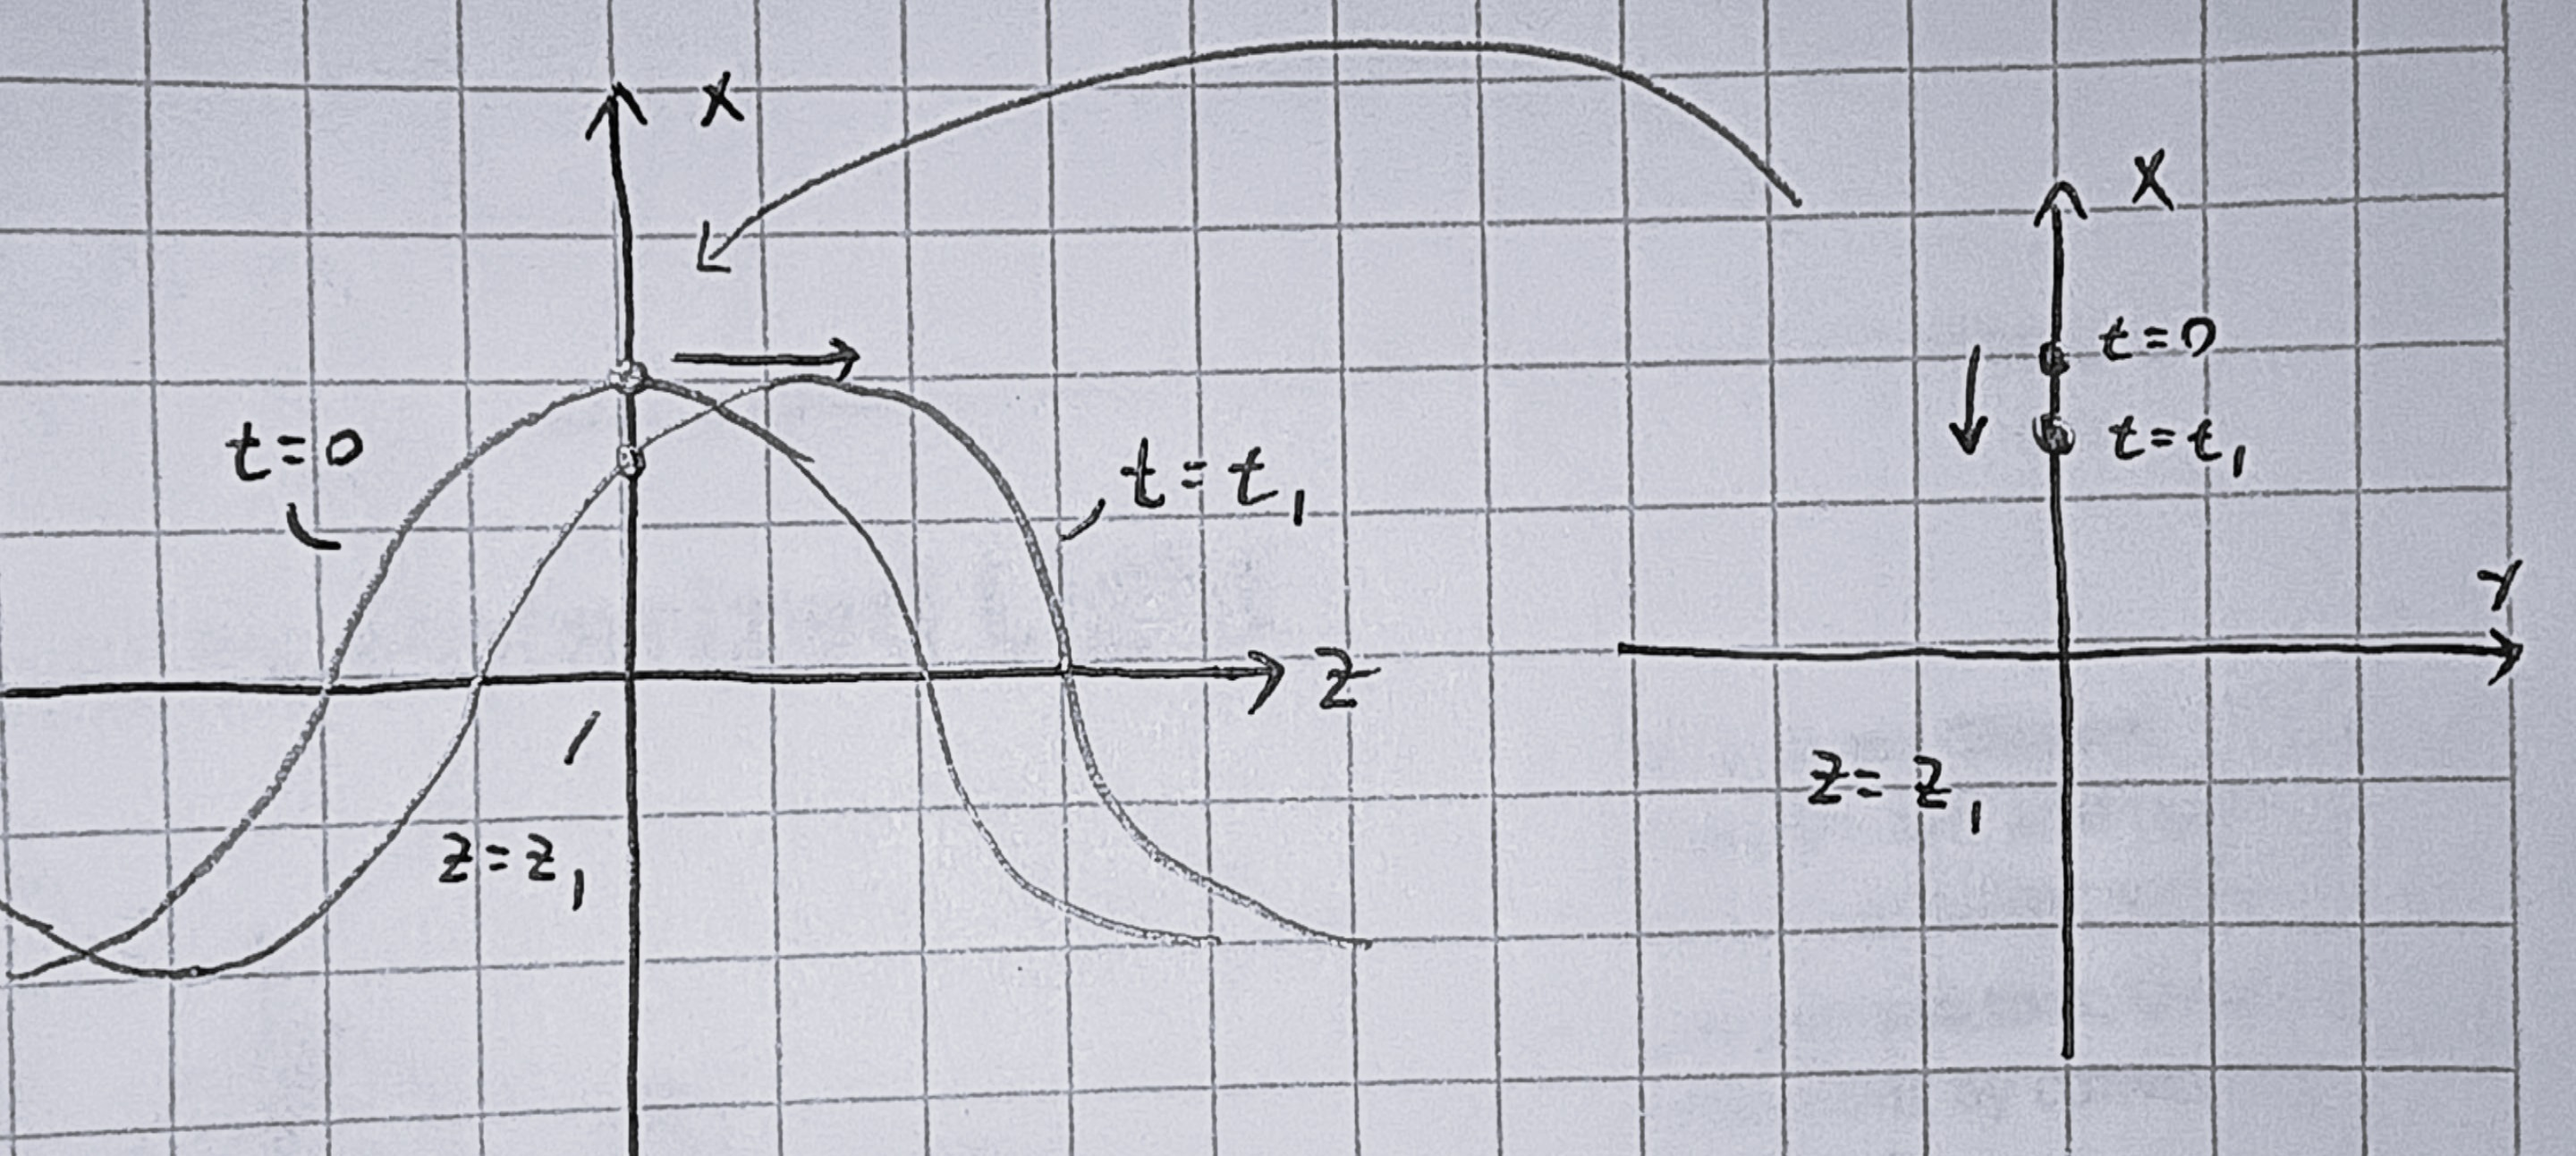
\includegraphics[width=0.5\textwidth]{Fixed z.jpg}
       \end{center}
       \item Fixing $t$, letting $z$ vary:\\
       Now imagine we are at a fixed time $t=t_1$. Moving along the $z$ axis, and plotting the wave’s amplitude, we see the full shape of the wave at that instant ($\omega t_1$ becomes a constant phase shift).
       \begin{center}
       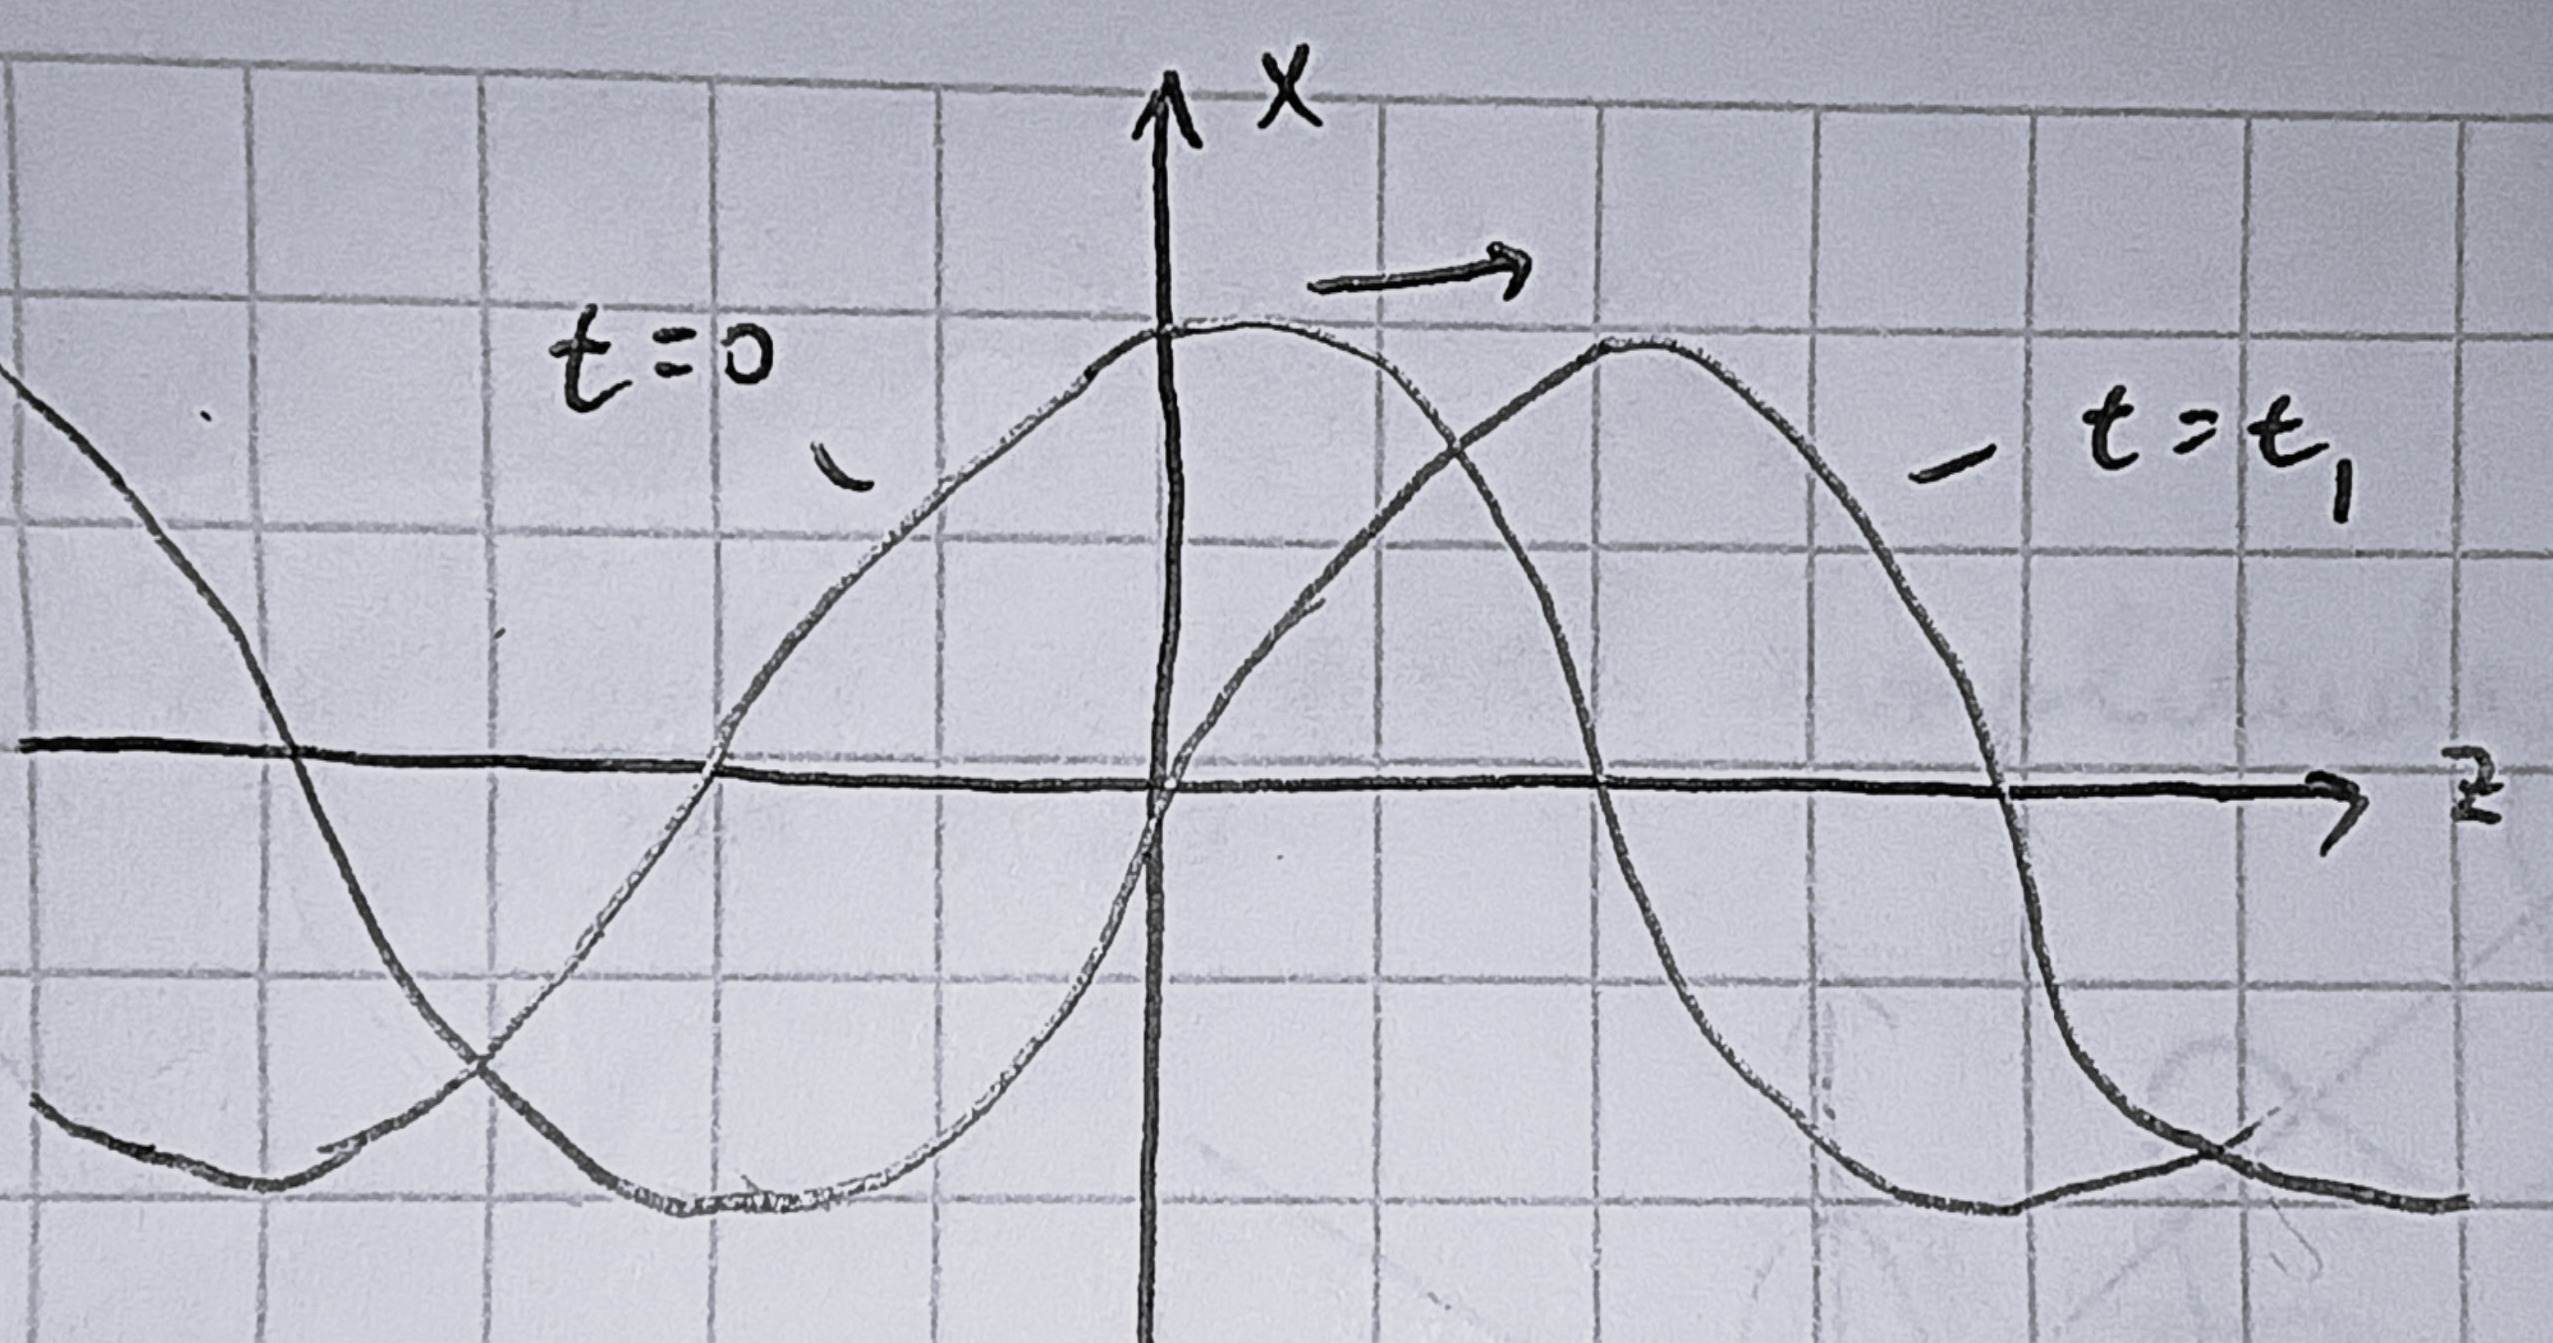
\includegraphics[width=0.5\textwidth]{Fixed t.jpg}
       \end{center}
       \item Letting $z$ and $t$ vary together:\\
       When we looked at $z$ and $t$ separately, we saw only a \textit{part} of the wave's behavior. For a fixed $z$, we observed how a single point moves over time, capturing the wave's temporal variation. For a fixed $t$, we saw the spatial variation, revealing the full shape of the wave statically at that instant. When both $z$ and $t$ vary together, we can see the wave's complete dynamic behavior, watching how its shape propagates through space and time.
       \begin{center}
       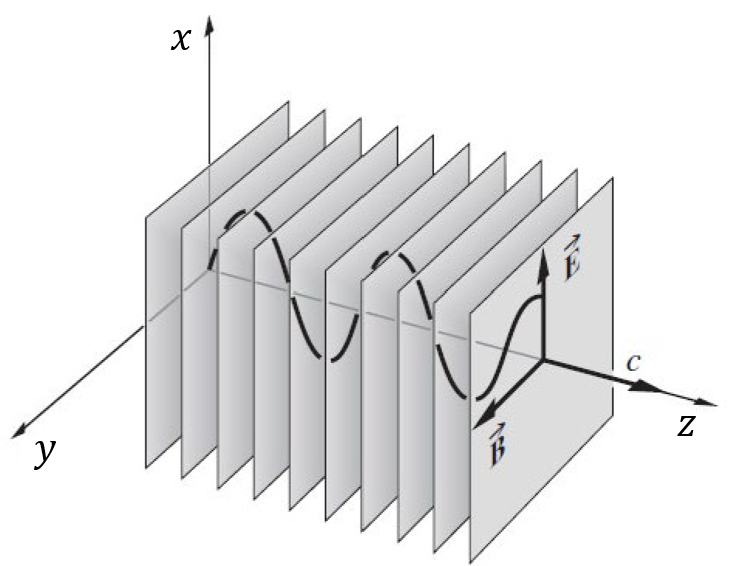
\includegraphics[width=0.5\textwidth]{Combined Views.png}
       \end{center}
\end{enumerate}
\underline{Note:} This intuition will become very useful when we study electromagnetic polarization, where the plane wave is a 2D wave. In our cross-sectional view, the single point along the wave will move along the $xy$ plane instead of just up and down.
\newpage
\section*{Vector Calculus}
\begin{itemize}
       \item \textbf{Del Operator:}
       \[\vec{\nabla} = \frac{\partial}{\partial x}\hat{x} + \frac{\partial}{\partial y}\hat{y} + \frac{\partial}{\partial z}\hat{z}\]
       \item \textbf{Laplacian Operator:} 
       \[\nabla^2 = \vec{\nabla} \cdot \vec{\nabla} = \frac{\partial^2}{\partial x^2} + \frac{\partial^2}{\partial y^2} + \frac{\partial^2}{\partial z^2} \quad \text{(in cartesian)}\]
       \item \textbf{Divergence:} Dot product of del operator with a vector field $\vec{A}$, giving a scalar field that represents how much $\vec{A}$ spreads (diverges) out from a point.
       \[\vec{\nabla} \cdot \vec{A} = \frac{\partial A_x}{\partial x} + \frac{\partial A_y}{\partial y} + \frac{\partial A_z}{\partial z}\]
       \underline{Note:} A positive divergence indicates a source, while a negative divergence indicates a sink.
       \item \textbf{Curl:} Cross product of del operator with a vector field $\vec{A}$, giving a vector field that represents how much $\vec{A}$ curls around a point.
\begin{align*}
\vec{\nabla} \times \vec{A}
&=
\begin{vmatrix}
\hat{x} & \hat{y} & \hat{z} \\
\frac{\partial}{\partial x} &
\frac{\partial}{\partial y} &
\frac{\partial}{\partial z} \\
A_x & A_y & A_z
\end{vmatrix} \\
&=
\underbrace{\left( \frac{\partial A_z}{\partial y}
- \frac{\partial A_y}{\partial z} \right)}_{\text{curl about }x\text{-axis}} \hat{x}
+
\underbrace{\left( \frac{\partial A_x}{\partial z}
- \frac{\partial A_z}{\partial x} \right)}_{\text{curl about }y\text{-axis}} \hat{y}
+
\underbrace{\left( \frac{\partial A_y}{\partial x}
- \frac{\partial A_x}{\partial y} \right)}_{\text{curl about }z\text{-axis}} \hat{z}
\end{align*}
\underline{Note:} A positive curl indicates a counterclockwise rotation, while a negative curl indicates a clockwise rotation about the respective axis.
\item \textbf{Vector Identities:} \\
\underline{Triple Products}
\begin{align*}
\vec{A} \cdot (\vec{B} \times \vec{C})
&= \vec{B} \cdot (\vec{C} \times \vec{A})
= \vec{C} \cdot (\vec{A} \times \vec{B}) \\
\vec{A} \times (\vec{B} \times \vec{C})
&= \vec{B}(\vec{A} \cdot \vec{C})
- \vec{C}(\vec{A} \cdot \vec{B})
\end{align*}
\underline{Product Rules}
\begin{align*}
\vec{\nabla}(fg) &= f(\vec{\nabla} g) + g(\vec{\nabla} f) \\
\vec{\nabla}(\vec{A} \cdot \vec{B})
&= \vec{A} \times (\vec{\nabla} \times \vec{B})
+ \vec{B} \times (\vec{\nabla} \times \vec{A})
+ (\vec{A} \cdot \vec{\nabla})\vec{B}
+ (\vec{B} \cdot \vec{\nabla})\vec{A} \\
\vec{\nabla} \cdot (f\vec{A})
&= f(\vec{\nabla} \cdot \vec{A}) + \vec{A} \cdot (\vec{\nabla} f) \\
\vec{\nabla} \cdot (\vec{A} \times \vec{B})
&= \vec{B} \cdot (\vec{\nabla} \times \vec{A})
- \vec{A} \cdot (\vec{\nabla} \times \vec{B}) \\
\vec{\nabla} \times (f\vec{A})
&= f(\vec{\nabla} \times \vec{A})
- \vec{A} \times (\vec{\nabla} f) \\
\vec{\nabla} \times (\vec{A} \times \vec{B})
&= (\vec{B} \cdot \vec{\nabla})\vec{A}
- (\vec{A} \cdot \vec{\nabla})\vec{B}
+ \vec{A}(\vec{\nabla} \cdot \vec{B})
- \vec{B}(\vec{\nabla} \cdot \vec{A}) 
\end{align*}
\underline{Second Derivatives}
\begin{align*}
\vec{\nabla} \cdot (\vec{\nabla} \times \vec{A}) &= 0 \quad \text{(Divergence of a curl is always zero)}\\
\vec{\nabla} \times (\vec{\nabla} f) &= 0 \quad \text{(Curl of a gradient is always zero)}\\
\vec{\nabla} \times (\vec{\nabla} \times \vec{A})
&= \vec{\nabla}(\vec{\nabla} \cdot \vec{A}) - \nabla^2 \vec{A} \quad\text{(Curl of a curl)}
\end{align*}
\end{itemize}
\section*{Divergence Theorem}
\begin{minipage}{0.5\textwidth}
Relates the flux of a vector field $\vec{F}$ through a closed surface $S$ to the divergence of $\vec{F}$ within the volume $V$ enclosed by $S$.
\[\underbrace{\int_{V} (\vec{\nabla} \cdot \vec{F}) \, d\tau}_{\text{how field spreads inside the volume}} = \underbrace{\oint_{S} \vec{F} \cdot d\vec{a}}_{\text{flux of field through the surface}}\]
\end{minipage}
\hfill
\begin{minipage}{0.4\textwidth}
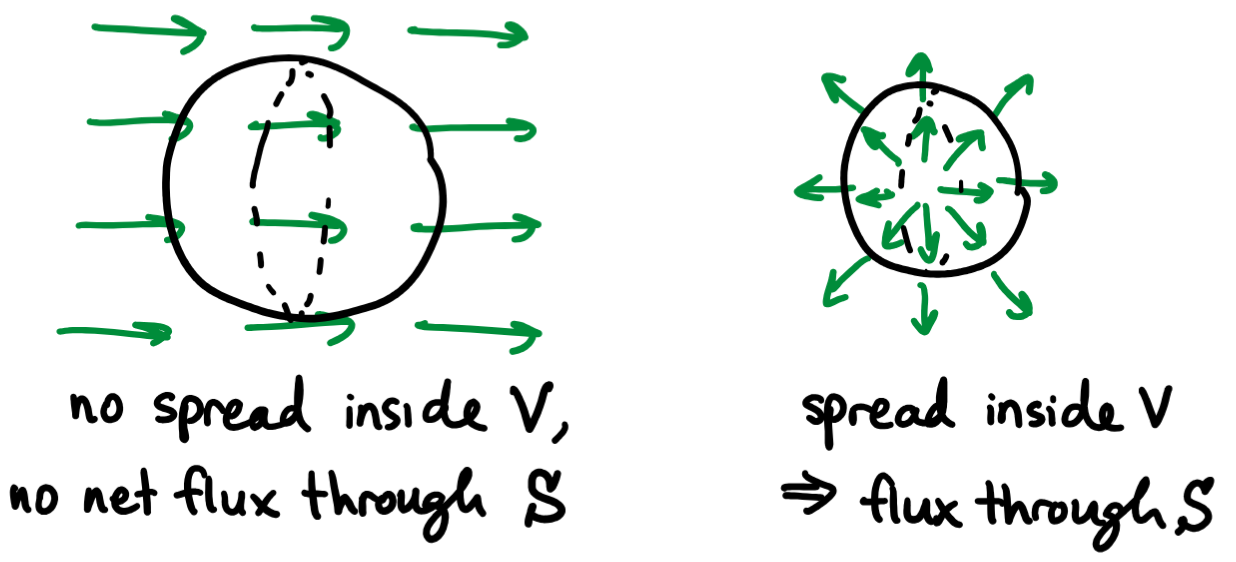
\includegraphics[width=\linewidth]{Divergence thm.png}
\end{minipage}
\section*{Stokes Theorem}
\begin{minipage}{0.5\textwidth}
States that inside a surface $A$ bounded by a closed curve $P$, if a vector field $\vec{F}$ has a non-zero curl \textit{about $\vec{A}$ (the normal to the surface)}, then there will be a non-zero circulation of $\vec{F}$ around the curve $P$.
\[\underbrace{\int_{A} (\vec{\nabla} \times \vec{F}) \cdot d\vec{a}}_{\text{flux of the curl of $\vec{F}$}} = \underbrace{\oint_{P} \vec{F} \cdot d\vec{l}}_{\text{circulation of $\vec{F}$}}\]
\end{minipage}
\hfill
\begin{minipage}{0.4\textwidth}
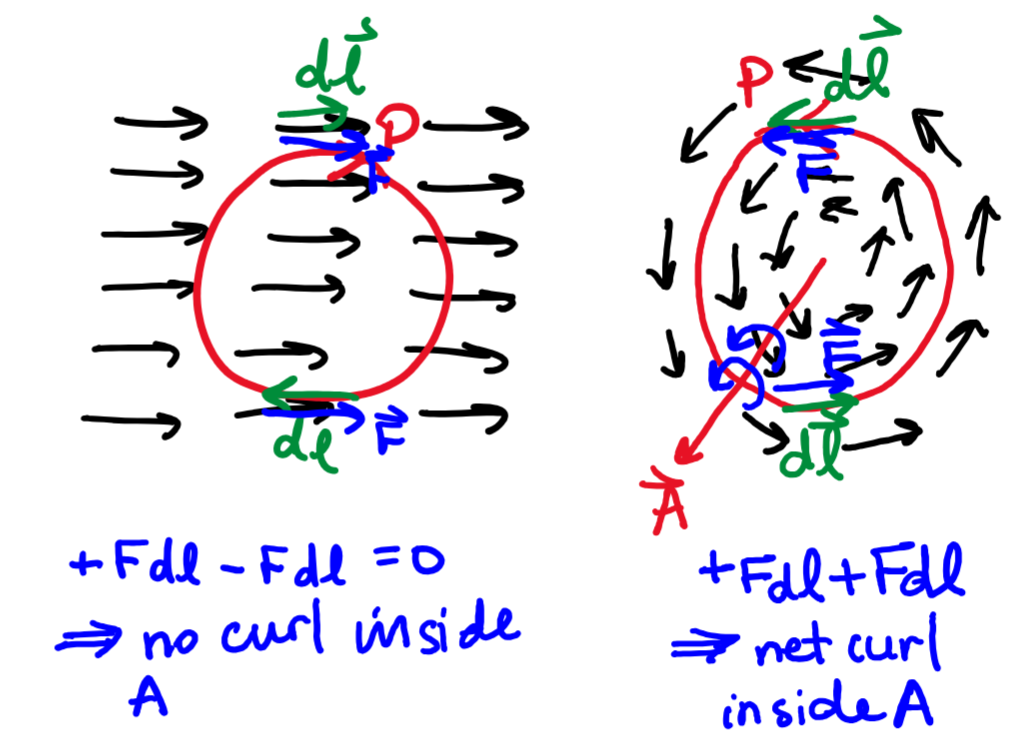
\includegraphics[width=\linewidth]{Stokes thm.png}
\end{minipage}
\section*{Key Electricity and Magnetism Laws}
\begin{multicols}{2}
\begin{itemize}
\item \textbf{Coulomb's Law} \[\vec{F}_{e} = \frac{1}{4 \pi \varepsilon_0} \frac{q_1 q_2}{r^2} \hat{r}\]
\item \textbf{Electric Field of a Point Charge}\\
sets up a diverging field \[\vec{E}=\frac{1}{4 \pi \varepsilon_0} \frac{q}{r^2} \hat{r}\]
\item \textbf{Magnetic Force} \[\vec{F}_b = q\vec{v}\times\vec{B}\]
\item \textbf{Biot-Savart Law}\\
sets up a curling field \[\vec{B} = \int \frac{\mu_0}{4\pi}\frac{i\,d\vec{s}\times\hat{r}}{r^2}\]
\end{itemize}
\end{multicols}
\vspace{1em}
\noindent\hrule
\vspace{1em}
\newpage
{\centering\LARGE Unit 1: Electromagnetic Waves\par}
\section*{Maxwell's Equations}
\begin{enumerate}
    \item \textbf{Gauss's Law for Electricity}\\
    Relates the electric flux through a closed 3D Gaussian surface to the total charge enclosed within that surface.
    \[\oint_S \vec{E}\cdot\,d\vec{a}=\frac{q_{\text{enc}}}{\varepsilon_0}\]
     There exists a diverging electric field if there exists a non-zero charge density at that point.
    \[\vec{\nabla}\cdot\vec{E}=\frac{\rho}{\varepsilon_0}\]

    \item \textbf{Gauss's Law for Magnetism}\\
    Any 3D Gaussian surface will have zero net magnetic flux (no magnetic monopoles).
    \[\oint_S \vec{B}\cdot\,d\vec{a}=0\]
    There exists no diverging magnetic field at any point in space because there are no magnetic monopoles.
    \[\vec{\nabla}\cdot\vec{B}=0\]

    \item \textbf{Faraday's Law of Induction}\\
    Relates the electric circulation around a closed Faradian loop to the changing magnetic flux through the surface bounded by the loop.    
    \[\oint_P \vec{E}\cdot d\vec{l}=-\frac{d\Phi_B}{dt}, \quad \Phi_B = \int_S \vec{B}\cdot\,d\vec{a}\]
    \underline{Note:} For coils with $N$ turns, multiply the flux by $N$.\\\\
    A changing magnetic field induces a circulating (curling) electric field.
    \[\vec{\nabla}\times\vec{E}=-\frac{\partial \vec{B}}{\partial t}\]

    \item \textbf{Ampere-Maxwell Law}\\
    Relates the magnetic circulation around a closed Amperian loop to the enclosed current and changing electric flux through the surface bounded by the loop.
    \[\oint_P \vec{B}\cdot d\vec{l}= \mu_0I_{\text{enc}}+\mu_0\varepsilon_0 \frac{d\Phi_E}{dt},\quad \Phi_E=\int_S \vec{E}\cdot\,d\vec{a}\]
    Both a changing electric field and a non-zero current density induce a circulating (curling) magnetic field.
    \[\vec{\nabla}\times\vec{B}= \mu_0\vec{J}+\mu_0\varepsilon_0 \frac{\partial \vec{E}}{\partial t}, \quad I_{\text{enc}}=\int_S \vec{J}\cdot d\vec{a}\]
\end{enumerate}
\section*{Deriving the Differential Forms of Maxwell's Equations}
By applying the divergence and stokes theorems to the integral forms of Maxwell's equations, we can derive their corresponding differential forms. This process allows us to express the behavior of electric and magnetic fields locally at every point in space and time, rather than just over closed surfaces or loops.
\begin{enumerate}
    \item \textbf{Gauss's Law for Electricity}
\[\oint_S \vec{E}\cdot\,d\vec{a}=\frac{q_{\text{enc}}}{\varepsilon_0}\]
Applying the divergence theorem to the left-hand side:
\[\oint_S \vec{E}\cdot\,d\vec{a}=\int_V (\vec{\nabla}\cdot\vec{E})\,d\tau\]
We can also write the enclosed charge as a volume integral of the charge density:
\[q_{\text{enc}}=\int_V \rho\,d\tau\,\quad \rho=\text{(vol charge density)}\]
Thus,
\[\implies \int_V (\vec{\nabla}\cdot\vec{E})\,d\tau = \frac{1}{\varepsilon_0} \int_V \rho\,d\tau\]
\[\implies \boxed{\vec{\nabla}\cdot\vec{E} = \frac{\rho}{\varepsilon_0}}\]

    \item \textbf{Gauss's Law for Magnetism}
\[\oint_S \vec{B}\cdot\,d\vec{a}=0\]
Applying the divergence theorem:
\[\oint_S \vec{B}\cdot\,d\vec{a}=\int_V (\vec{\nabla}\cdot\vec{B})\,d\tau = 0\]
Thus,
\[\implies \boxed{\vec{\nabla}\cdot\vec{B} = 0}\]

    \item \textbf{Faraday's Law of Induction}
\[\oint_P \vec{E}\cdot d\vec{l}=-\frac{d\Phi_B}{dt}, \quad \Phi_B = \int_S \vec{B}\cdot\,d\vec{a}\]
Applying Stokes' theorem to the left-hand side:
\[\oint_P \vec{E}\cdot d\vec{l} = \int_S (\vec{\nabla}\times\vec{E})\cdot d\vec{a}\]
We can also write the changing magnetic flux as:
\[-\frac{d\Phi_B}{dt} = -\frac{d}{dt}\left[\int_S \vec{B}\cdot\,d\vec{a}\right] =-\int_S \frac{\partial \vec{B}}{\partial t}\cdot d\vec{a}\]
\underline{Note:} Stokes theorem relates the circulation around a curve to the curl over a surface at a single instant in time. In other words, the surface $S$ is \textit{fixed} and does not change in time, so $d\vec{a}$ is \textit{time independent} and the time derivative acts only on the integrand, allowing us to move the time derivative inside the integral.\\\\
Thus, equating the two sides gives:
\[\implies \int_S (\vec{\nabla}\times\vec{E})\cdot d\vec{a} = -\int_S \frac{\partial \vec{B}}{\partial t}\cdot d\vec{a}\]
\[\implies \boxed{\vec{\nabla}\times\vec{E} = -\frac{\partial \vec{B}}{\partial t}}\]
    \item \textbf{Ampere-Maxwell Law}
\[\oint_P \vec{B}\cdot d\vec{l}= \mu_0I_{\text{enc}}+\mu_0\varepsilon_0 \frac{d\Phi_E}{dt},\quad \Phi_E=\int_S \vec{E}\cdot\,d\vec{a}\]
Applying Stokes' theorem to the left-hand side:
\[\oint_P \vec{B}\cdot d\vec{l} = \int_S (\vec{\nabla}\times\vec{B})\cdot d\vec{a}\]
We can also write the enclosed current as a surface integral of the current density:
\[I_{\text{enc}}=\int_S \vec{J}\cdot d\vec{a}, \quad \vec{J}=\text{(area current density)}\]
And the changing electric flux as:
\[\frac{d\Phi_E}{dt} = \frac{d}{dt}\left[\int_S \vec{E}\cdot\,d\vec{a}\right] = \int_S \frac{\partial \vec{E}}{\partial t}\cdot d\vec{a}\]
Thus, equating the two sides gives:
\[\implies \int_S (\vec{\nabla}\times\vec{B})\cdot d\vec{a} = \int_S \left(\mu_0\vec{J}+\mu_0\varepsilon_0 \frac{\partial \vec{E}}{\partial t}\right)\cdot d\vec{a}\]
\[\implies \boxed{\vec{\nabla}\times\vec{B} = \mu_0\vec{J}+\mu_0\varepsilon_0 \frac{\partial \vec{E}}{\partial t}}\]
\end{enumerate}
\newpage\noindent
\textbf{Applying Vector Identities}\\
Additionally, we can apply the vector identities we have to the differential forms of Maxwell's equations to derive some useful results.\\\\
\underline{Applying divergence of a curl is zero to Faraday's law:}
\begin{align*}
    \vec{\nabla}\cdot(\vec{\nabla}\times\vec{E}) &= 0 \\
\quad \vec{\nabla}\cdot\left(-\frac{\partial \vec{B}}{\partial t}\right) &= 0\\
    -\frac{\partial}{\partial t} \underbrace{(\nabla \cdot \vec{B})\rule[-10pt]{0pt}{0pt}}_{\mathclap{\text{Gauss's law for magnetism } (=0)}} &= 0 \\
    \implies 0 &= 0
\end{align*}
\underline{Applying divergence of a curl is zero to Ampere-Maxwell law:}
\begin{align*}
    \vec{\nabla}\cdot(\vec{\nabla}\times\vec{B}) &= 0 \\
    \quad \vec{\nabla}\cdot\left(\mu_0\vec{J}+\mu_0\varepsilon_0 \frac{\partial \vec{E}}{\partial t}\right) &= 0 \\
    \mu_0(\vec{\nabla}\cdot\vec{J}) + \mu_0\varepsilon_0 \frac{\partial}{\partial t} \underbrace{(\nabla \cdot \vec{E}) \rule[-10pt]{0pt}{0pt}}_{\mathclap{\text{Gauss's law for electricity}(=\frac{\rho}{\varepsilon_0})}} &= 0 \\
    \mu_0(\vec{\nabla}\cdot\vec{J}) + \mu_0\varepsilon_0 \frac{\partial}{\partial t} \left(\frac{\rho}{\varepsilon_0}\right) &= 0
\end{align*}
\[\implies \boxed{\vec{\nabla}\cdot\vec{J} + \frac{\partial \rho}{\partial t} = 0}\quad \text{(Continuity Equation)}\]
We can rewrite the continuity equation into an integral form:\\\\
Integrating both sides over a volume $V$:
\[\int_V (\vec{\nabla} \cdot \vec{J}) \, d\tau = \int_V - \frac{\partial \rho}{\partial t} \, d\tau\]
Apply divergence theorem to the left-hand side:
\[\int_V (\vec{\nabla} \cdot \vec{J}) \, d\tau = \oint_S \vec{J} \cdot d\vec{a}\]
Since the volume $V$ is fixed in space, we can pull the time derivative outside the integral. We also know that the total charge enclosed is $q = \int_V \rho \, d\tau$:
\[\int_V - \frac{\partial \rho}{\partial t} \, d\tau = - \frac{d}{dt} \underbrace{\int_V \rho \, d\tau}_{q_{\text{enclosed}}} = - \frac{dq}{dt}\]
Thus, equating the two sides gives:
\[\boxed{\oint_S \vec{J}\cdot\,d\vec{a} = -\frac{dq}{dt}}\]
\underline{Note:} The continuity equation is also called a flux based conservation law. It represents a local \textbf{conservation of charge} and states that if the total charge enclosed in a volume is changing ($\frac{dq}{dt} \neq 0$), then there must be a net current flowing into or out of the volume ($\oint_S \vec{J}\cdot\,d\vec{a} \neq 0$) that accounts for that change.
\begin{center}
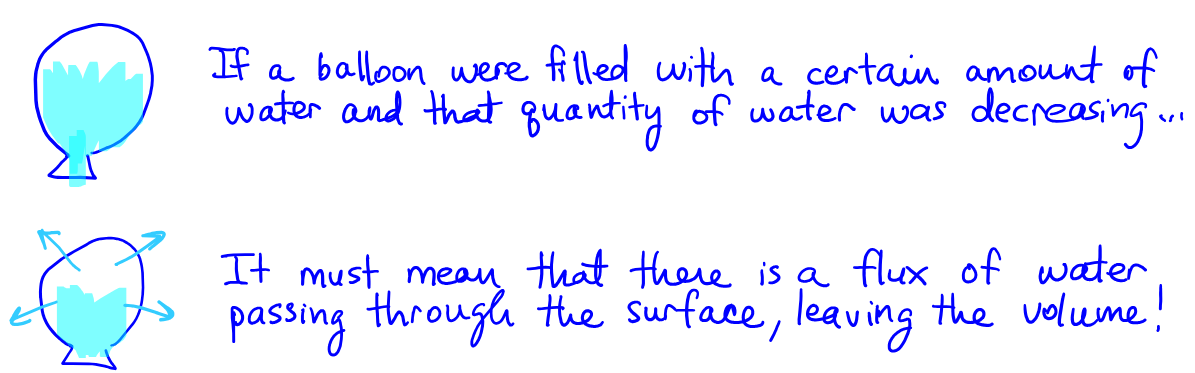
\includegraphics[width=0.8\textwidth]{Continuity.png}
\end{center}
\textbf{Showing that E and B Fields Exist as Waves in a Vacuum}\\
In a vacuum, there are no charges or currents, so we can set $\rho = 0$ and $\vec{J} = \vec{0}$ in Maxwell's equations. This simplifies them to:
\[\boxed{
\begin{aligned}
  \vec{\nabla} \cdot \vec{E} &= 0 
  &\qquad
  \vec{\nabla} \cdot \vec{B} &= 0 
  &\qquad
  &\text{no divergent fields (no source charge)} \\[1em]
  \vec{\nabla} \times \vec{E} &= -\frac{\partial \vec{B}}{\partial t} 
  &\qquad
  \vec{\nabla} \times \vec{B} &= \mu_0 \varepsilon_0 \frac{\partial \vec{E}}{\partial t} 
  &\qquad
  &\text{only exist curling fields induced by one another!}
\end{aligned}}\]
By applying the curl of a curl rule to Faraday's and Ampere-Maxwell laws, we can derive the wave equations for the electric and magnetic fields in a vacuum.\\
\begin{minipage}{0.45\textwidth}
\begin{align*}
    \vec{\nabla} \times (\vec{\nabla} \times \vec{E}) &= \vec{\nabla}(\underbrace{\vec{\nabla} \cdot \vec{E}\rule[-5pt]{0pt}{0pt}}_{\mathclap{0 \text{ in a vacuum}}}) - \nabla^2 \vec{E} \\
    \vec{\nabla} \times \left(-\frac{\partial \vec{B}}{\partial t}\right) &= - \nabla^2 \vec{E} \\
    -\frac{\partial}{\partial t} (\vec{\nabla} \times \vec{B}) &= - \nabla^2 \vec{E} \\
    -\frac{\partial}{\partial t} \left(\mu_0 \varepsilon_0 \frac{\partial \vec{E}}{\partial t}\right) &= - \nabla^2 \vec{E} \\[1em]
    \implies \boxed{\nabla^2 \vec{E} = \mu_0 \varepsilon_0 \frac{\partial^2 \vec{E}}{\partial t^2}}
\end{align*}
\end{minipage}
\hfill
\begin{minipage}{0.45\textwidth}
\begin{align*}
    \vec{\nabla} \times (\underbrace{\vec{\nabla} \times \vec{B}\rule[-5pt]{0pt}{0pt}}_{\mathclap{\mu_0 \varepsilon_0 \frac{\partial \vec{E}}{\partial t}\, \text{in a vacuum}}}) &= \vec{\nabla}(\underbrace{\vec{\nabla} \cdot \vec{B}\rule[-5pt]{0pt}{0pt}}_{0}) - \nabla^2 \vec{B} \\[1em]
    \mu_0 \varepsilon_0 \frac{\partial}{\partial t} (\underbrace{\vec{\nabla} \times \vec{E}\rule[-5pt]{0pt}{0pt}}_{-\frac{\partial \vec{B}}{\partial t}}) &= - \nabla^2 \vec{B} \\
    -\mu_0 \varepsilon_0 \frac{\partial^2 \vec{B}}{\partial t^2} &= - \nabla^2 \vec{B} \\[1em]
    \implies \boxed{\nabla^2 \vec{B} = \mu_0 \varepsilon_0 \frac{\partial^2 \vec{B}}{\partial t^2}}
\end{align*}
\end{minipage}\\\\
\underline{Recall:} The classic wave equation is 
\[\nabla^2 \psi = \frac{1}{v^2} \frac{\partial^2 \psi}{\partial t^2}\quad \implies \quad v = \frac{1}{\sqrt{\mu_0 \varepsilon_0}} = c\]
\section*{Modeling EM Radiation (Light) in a Vacuum}
Properties of light:
\begin{itemize}
       \item $\vec{E}\times\vec{B}$ points in the direction of propagation.
       \item $\vec{E}$ and $\vec{B}$ are perpendicular to each other and to the direction of propagation (transverse wave).
       \item $\vec{E}$ and $\vec{B}$ oscillate in phase as to perpetually induce each other according to Faraday's and Ampere-Maxwell laws.
       \item The magnitudes of $\vec{E}$ and $\vec{B}$ are related by $E = cB$.
       \item Light does not require a medium to propagate.
       \item Light has speed
       \[v = c = \frac{1}{\sqrt{\mu_0 \varepsilon_0}}\]
\end{itemize}
Our goal is to find a solution for $\vec{E}$ and $\vec{B}$ that satisfies the 3D wave equations as well as Maxwell's equations in a vacuum.\\\\
\textbf{Plane Wave Approximation}\\
Consider the following wavefronts generated by a point source of light (ie. a star):
\begin{center}
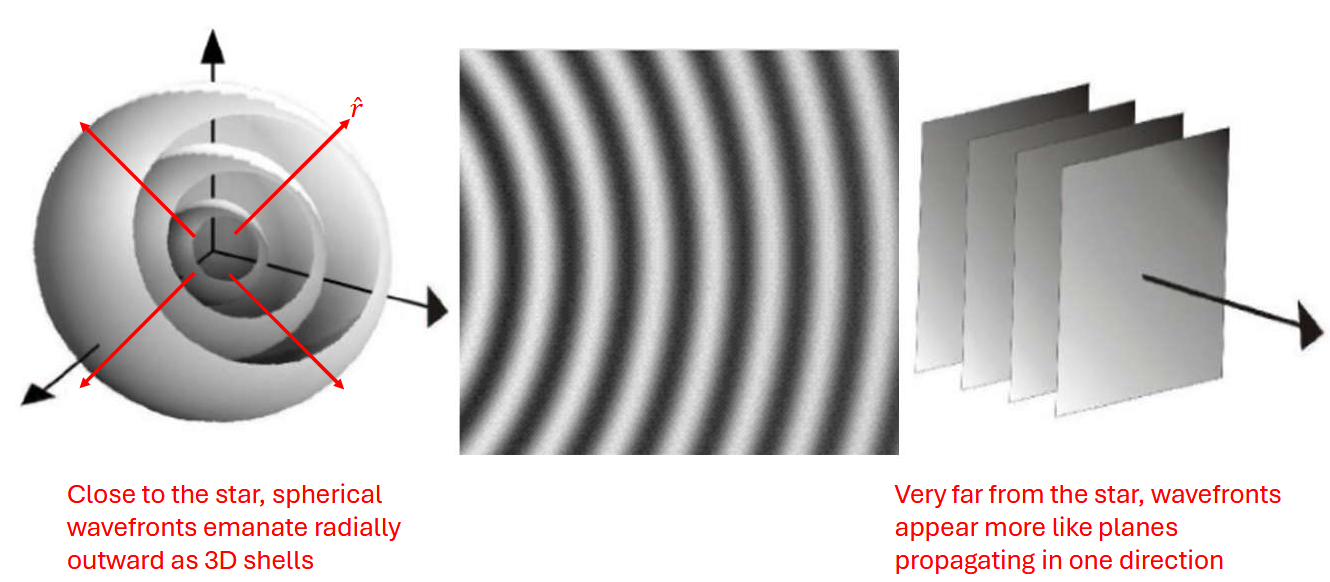
\includegraphics[width=0.8\textwidth]{Plane Wave.png}
\end{center}
The radius of curvature of the wavefronts increases as they travel outward. Thus, at a far enough distance from the source, the wavefronts will appear to be flat planes consisting of electric and magnetic fields with \textit{uniform} magnitude and direction. This is called the \textbf{plane wave approximation}.\\\\
The plane wave model also assumes \textbf{monochromatic light}, having a fixed wavelength $\lambda$ and wavenumber $k$ ($k = 2\pi/\lambda$). This also implies a fixed frequency $\omega$, since the speed of light is constant:
\[
v = \frac{\omega}{k} = c \quad \implies \quad \omega = c k.
\]
Without a single frequency, the wavefronts would interfere with one another and would no longer form the ideal uniform planes described by the plane wave approximation.
\begin{center}
\begin{minipage}{0.49\textwidth}
    \centering
    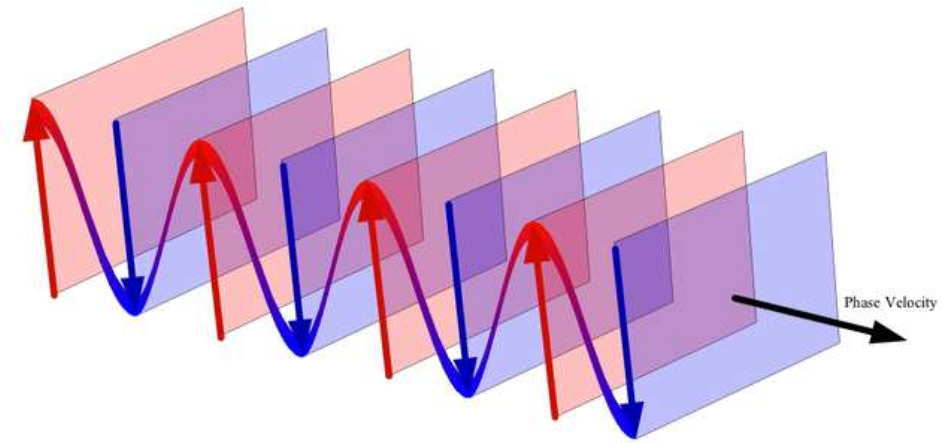
\includegraphics[width=\textwidth]{Plane Wave 1.png}
\end{minipage}
\hfill
\begin{minipage}{0.49\textwidth}
    \centering
    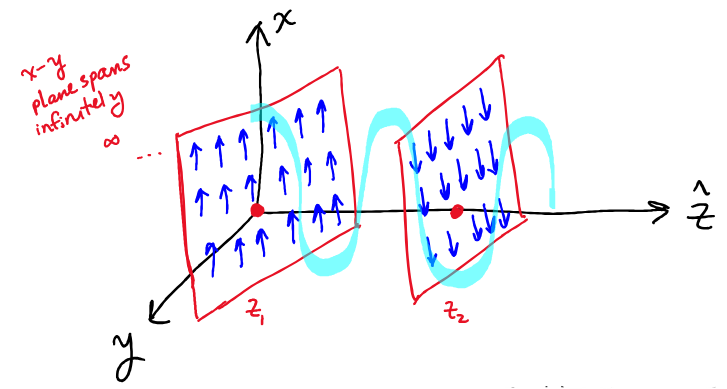
\includegraphics[width=\textwidth]{Plane Wave 2.png}
\end{minipage}
\end{center}
\underline{Note:} Although light consists of both electric and magnetic fields, we will primarily focus on the electric field when modeling light, since the magnetic field can be readily derived from it using Faraday’s law. We will also focus on the electric field when analyzing polarization, since the direction of the electric field determines the polarization of light.\\\\
\textbf{Case $\hat{z}$}\\
For the case $\hat{z}$, we take the direction of propagation to be along the $+z$ axis. At any fixed position $z$, the electric field $\vec{E}$ has a uniform magnitude and direction across the entire $xy$ plane. As with the 1D plane wave, the \textit{local view} at a fixed point along the $z$ axis shows the electric field oscillating in time as the light wave passes through, with the electric field remaining transverse to the direction of propagation.\\\\
\underline{Note:} Don't forget that the magnetic field $\vec{B}$ is also oscillating in phase with and is perpendicular to both $\vec{E}$ and the direction of propagation.
\vspace{-.5em}
\begin{center}
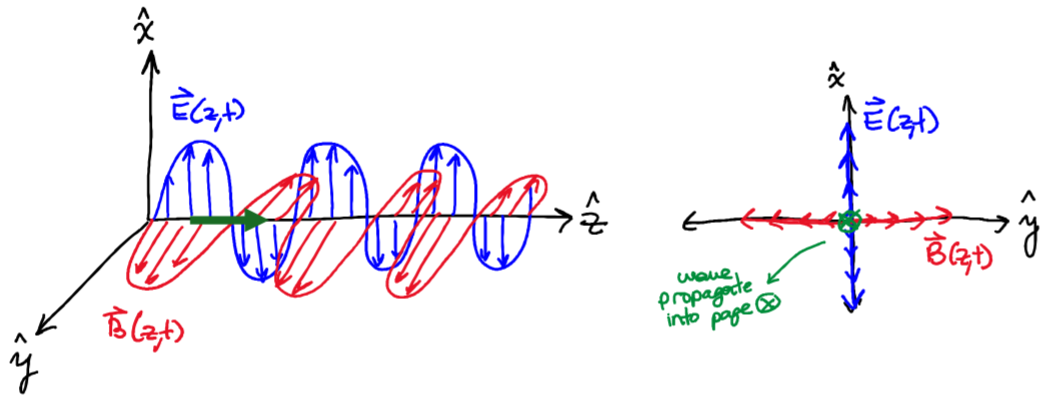
\includegraphics[width=0.8\textwidth]{Plane Wave 3.png}
\end{center} \vspace{-1em}
Therefore, a solution for the electric field of a plane wave in case $\hat{z}$ is:
\[\boxed{\vec{E} = \underbrace{\left( E_{0_x} e^{i \phi_x} \hat{x} + E_{0_y} e^{i \phi_y} \hat{y} \right)}_{\text{complex amplitude vector}} e^{i (k z - \omega t)}}\]
From the equation, we can see that the magnitudes of the electric field in the $x$ and $y$ directions need not be the same, and that there is no $z$ component of the electric field, since the wave is transverse. Like the 1D plane wave, the space and time dependence of this 3D plane wave is contained in the phase $(kz - \omega t)$.\\\\
The amplitude of the electric field is given by
\[|\vec{E}| = \sqrt{|E_{0_x}|^2 + |E_{0_y}|^2}\]
\underline{Note:} The phases $\phi_x$ and $\phi_y$ of the complex amplitude vector do not affect the magnitude of the electric field, but they do govern the polarization of the light wave. This is because of the dot product:
\[|\vec{E}|^2 = \vec{E}\cdot\vec{E}^*,\quad \vec{E}^*=\text{(complex conjugate of $\vec{E}$)}\]
\[\vec{E}\cdot\vec{E}^* = \left( E_{0_x} e^{i \phi_x} \hat{x} + E_{0_y} e^{i \phi_y} \hat{y} \right) \cdot \left( E_{0_x} e^{-i \phi_x} \hat{x} + E_{0_y} e^{-i \phi_y} \hat{y} \right) = |E_{0_x}|^2 + |E_{0_y}|^2\]
The exponentials multiply to 1 ($e^0$), and $\hat{x}\cdot\hat{x} = \hat{y}\cdot\hat{y} = 1$, while $\hat{x}\cdot\hat{y} = \hat{y}\cdot\hat{x} = 0$, so the cross terms cancel out.\\\\
\underline{Note:} The $xy$ components for both the electric and magnetic fields have the same harmonic properties of $k$ and $\omega$ (wavelength and frequency), since they are both derived from the same phase $(kz - \omega t)$.\\\\
Finally, note that we have switched from sinusoidal functions to complex exponentials. This is because complex exponentials are easier to work with mathematically, and if we want to get back to the real-valued (physically measurable) electric field, we can simply take the real part of the complex expression (using Euler's formula).
\[
\vec{E}_{\text{real}} = \Re\! \Big\{ \vec{E} \Big\} 
= \Re\! \Big\{ \big( E_{0_x} e^{i \phi_x} \hat{x} + E_{0_y} e^{i \phi_y} \hat{y} \big) e^{i (k z - \omega t)} \Big\}
\]
\[
\vec{E}_{\text{real}} = 
E_{0_x} \cos(k z - \omega t + \phi_x)\,\hat{x}
+ E_{0_y} \cos(k z - \omega t + \phi_y)\,\hat{y}
\]
\section*{Polarization of Light}
Polarization has been mentioned a few times already, but what exactly is it? Simply put, polarization describes the path traced out by the tip of the electric field vector $\vec{E}$ in the $xy$ plane at a fixed $z$ as the light wave passes through it. How can we visualize this? With \textit{parametric equations}.\\\\
First, to better understand the phase difference between the $x$ and $y$ components of the electric field, we draw a phasor diagram in the complex plane:
\begin{center}

\includegraphics[width=0.8\textwidth]{Phasor.jpg}
\end{center}
Where
\[E_x = E_{0_x}e^{i (\phi_x+ k z_1 - \omega t)}\]
\[E_y = E_{0_y}e^{i (\phi_y+ k z_1 - \omega t)}\]
\[\boxed{\varepsilon = \phi_x-\phi_y\quad \text{(phase difference)}}\]
Since $z = z_1$ is fixed, $kz_1$ becomes a constant phase offset, so the rotation of the phasors is driven entirely by $-\omega t$ (CW, since it is negative). The phase $kz_1 - \omega t$ is the same for both $E_x$ and $E_y$, so the relative phase difference $\varepsilon$ between the two components remains constant as the light wave propagates. Also note that while the magnitudes of $E_x$ and $E_y$ are constant in the phasor diagram, their \textit{real} magnitudes are given by the projections of the phasors onto the real axis, which oscillate in time (allowing elliptical polarization, where the magnitude of $\vec{E}$ varies in time).\\\\
\textbf{General Polarization}\\
The most general case of polarization is elliptical polarization, where linear and circular polarization are just degenerate ellipses. To see this, we will rewrite the \textit{real} electric field components in terms of the phase difference $\varepsilon$:
\[\vec{E}_{\text{real}} = 
E_{0_x} \cos(k z_1 - \omega t + \phi_x)\,\hat{x}
+ E_{0_y} \cos(k z_1 - \omega t + \phi_y)\,\hat{y}\]
\vspace{-3em}
\begin{align*}
    x(t) &= E_{0_x} \cos(\omega t - \varepsilon) \\
    y(t) &= E_{0_y} \cos(\omega t)
\end{align*}
\underline{Note:} $kz_1$ is constant, so it cancels out when we take the difference of the two phases, but we keep $\omega t$ in the argument since it is the time-varying part. Because we define $\varepsilon$ to be positive, it appears in the $x$ component (which is why $E_x$ leads $E_y$ in the phasor diagram). The argument of the cosine is $\varepsilon - \omega t$, but since cosine is an even function, we can equivalently write it as $\omega t - \varepsilon$.\\\\
We now deparametrize the equations to obtain a single equation in $x$ and $y$ that describes the path traced out by $\vec{E}$ in the $xy$ plane. First expanding the cosine using sum and difference:
\begin{align*}
    x(t) &= E_{0_x}(\cos(\omega t)\cos(\varepsilon) + \sin(\omega t)\sin(\varepsilon)) \\
    y(t) &= E_{0_y} \cos(\omega t) \implies \cos(\omega t) = \frac{y}{E_{0_y}}
\end{align*}
Substituting $\cos(\omega t)$ into the $x$ equation:
\[x(t) = E_{0_x}\left(\frac{y}{E_{0_y}}\cos(\varepsilon) + \sin(\omega t)\sin(\varepsilon)\right)\]
Solving for $\sin(\omega t)$:
\[\sin(\omega t) = \frac{1}{\sin(\varepsilon)}\left(\frac{x}{E_{0_x}} - \frac{y}{E_{0_y}}\cos(\varepsilon)\right)\]
Plugging $\sin(\omega t)$ and $\cos(\omega t)$ into the Pythagorean identity $\cos^2(\omega t) + \sin^2(\omega t) = 1$:
\[\left(\frac{y}{E_{0_y}}\right)^2+\left(\frac{1}{\sin(\varepsilon)}\left(\frac{x}{E_{0_x}} - \frac{y}{E_{0_y}}\cos(\varepsilon)\right)\right)^2=1\]
Simplify:
\[\boxed{\frac{x^2}{E_{0_x}^2}+\frac{y^2}{E_{0_y}^2}-2\frac{xy}{E_{0_x}E_{0_y}}\cos(\varepsilon) = \sin^2(\varepsilon)}\]
\underline{Note:} This is the form of an ellipse centered at the origin ($ax^2 +bxy +cy^2 = d$)\\\\
Therefore, for any $\varepsilon$ that doesn't result in a degenerate case, the polarization of light is elliptical. Now we will list some cases so we don't have to keep referring back to the general equation:
\begin{itemize}
    \item \textbf{Linear Polarization:} $E_x$ and $E_y$ are in phase and the ratio of their magnitudes is constant (slope of the line).
\[\boxed{\varepsilon = n\pi,\quad n=(0,1,2,\dots)}\]
\begin{center}
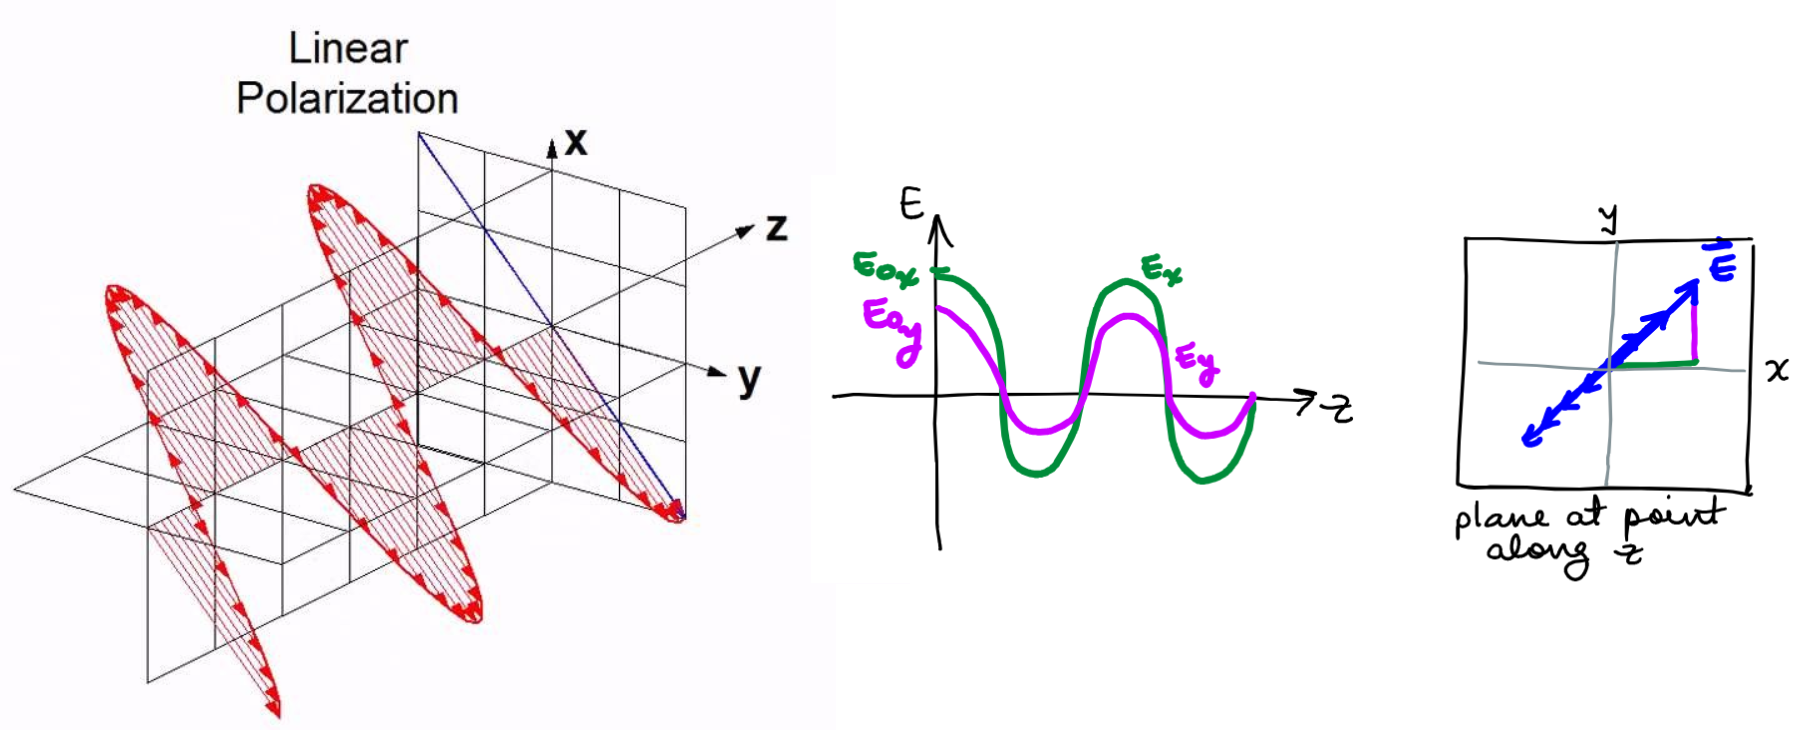
\includegraphics[width=0.8\textwidth]{Linear Polarization.png}
\end{center}
    \item \textbf{Circular Polarization:} $E_x$ and $E_y$ have equal magnitudes and are $\pi/2$ out of phase.
\[\boxed{E_{0_x} = E_{0_y},\quad \text{and} \quad \varepsilon = (2n+1)\frac{\pi}{2}, \quad n=(0,1,2,\dots)}\]
\begin{center}
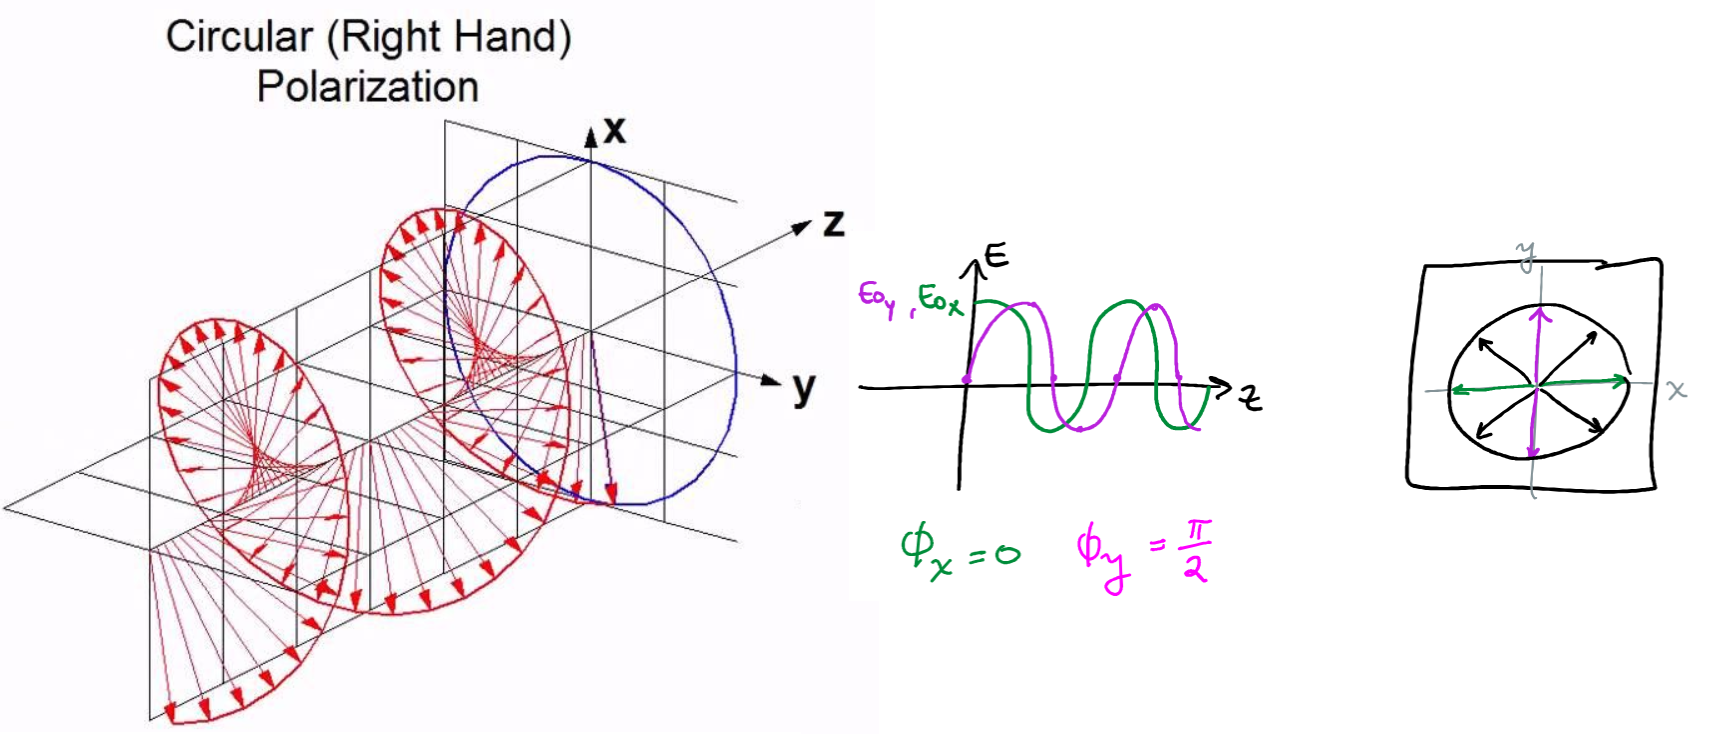
\includegraphics[width=0.8\textwidth]{Circular Polarization.png}
\end{center}
\newpage
    \item \textbf{Elliptical Polarization:} All other cases
\[\boxed{E_{0_x}\neq E_{0_y}, \quad \text{and} \quad \varepsilon \neq n\pi \quad \text{(otherwise it will be linear)}}\]
\begin{center}
OR
\end{center}
\[\boxed{E_{0_x} = E_{0_y}, \quad \text{and} \quad \varepsilon \neq (2n+1)\frac{\pi}{2} \quad \text{(otherwise it will be circular)}}\]
\begin{center}
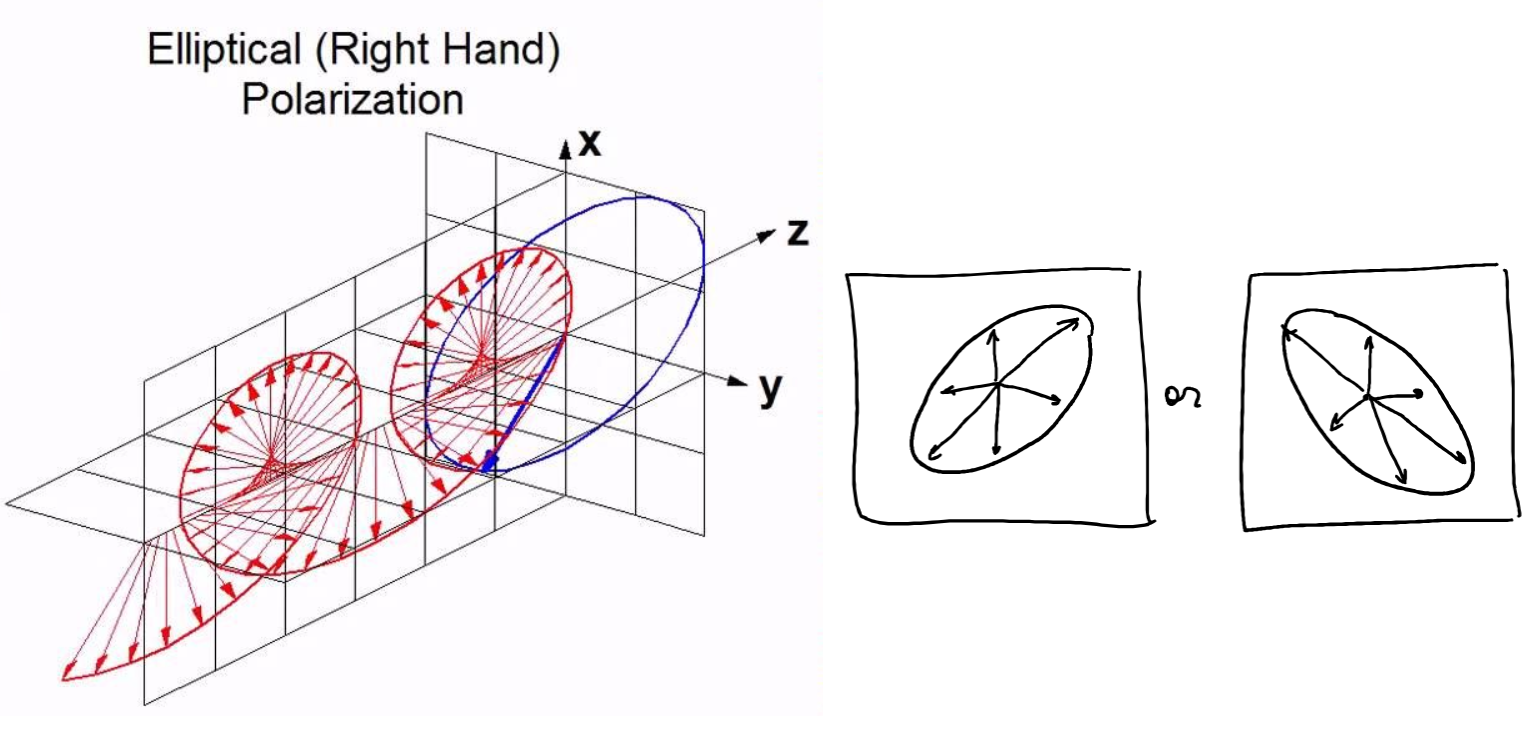
\includegraphics[width=0.6\textwidth]{Elliptical Polarization.png}
\end{center}
\end{itemize}
\textbf{Why Ellipses?}\\
Fundamentally, the electric and magnetic fields behave like oscillators, so the path traced out by the electric field vector must be periodic and closed. The only conic section that is both periodic and closed is an ellipse, with circles and lines appearing as degenerate cases. Another way to visualize this is to think of $E_x$ and $E_y$ as two simple harmonic oscillators (SHOs) that are coupled through a common driving frequency, analogous to two springs with equal spring constant $k$ attached to the same mass. The motion of the mass is then a superposition of the two SHOs, and the resulting path traced out by the mass is an ellipse. Feynman also introduces the picture of a string-mass pendulum, where the mass can swing in any direction in the $xy$ plane, and the path traced out by the mass is likewise an ellipse. This intuition is useful because it emphasizes that the driving phase $\omega t$ is the same for both the $x$ and $y$ components, and that the phase difference, and thus the resulting trace, depends only on the initial orientation of the motion.
\begin{center}
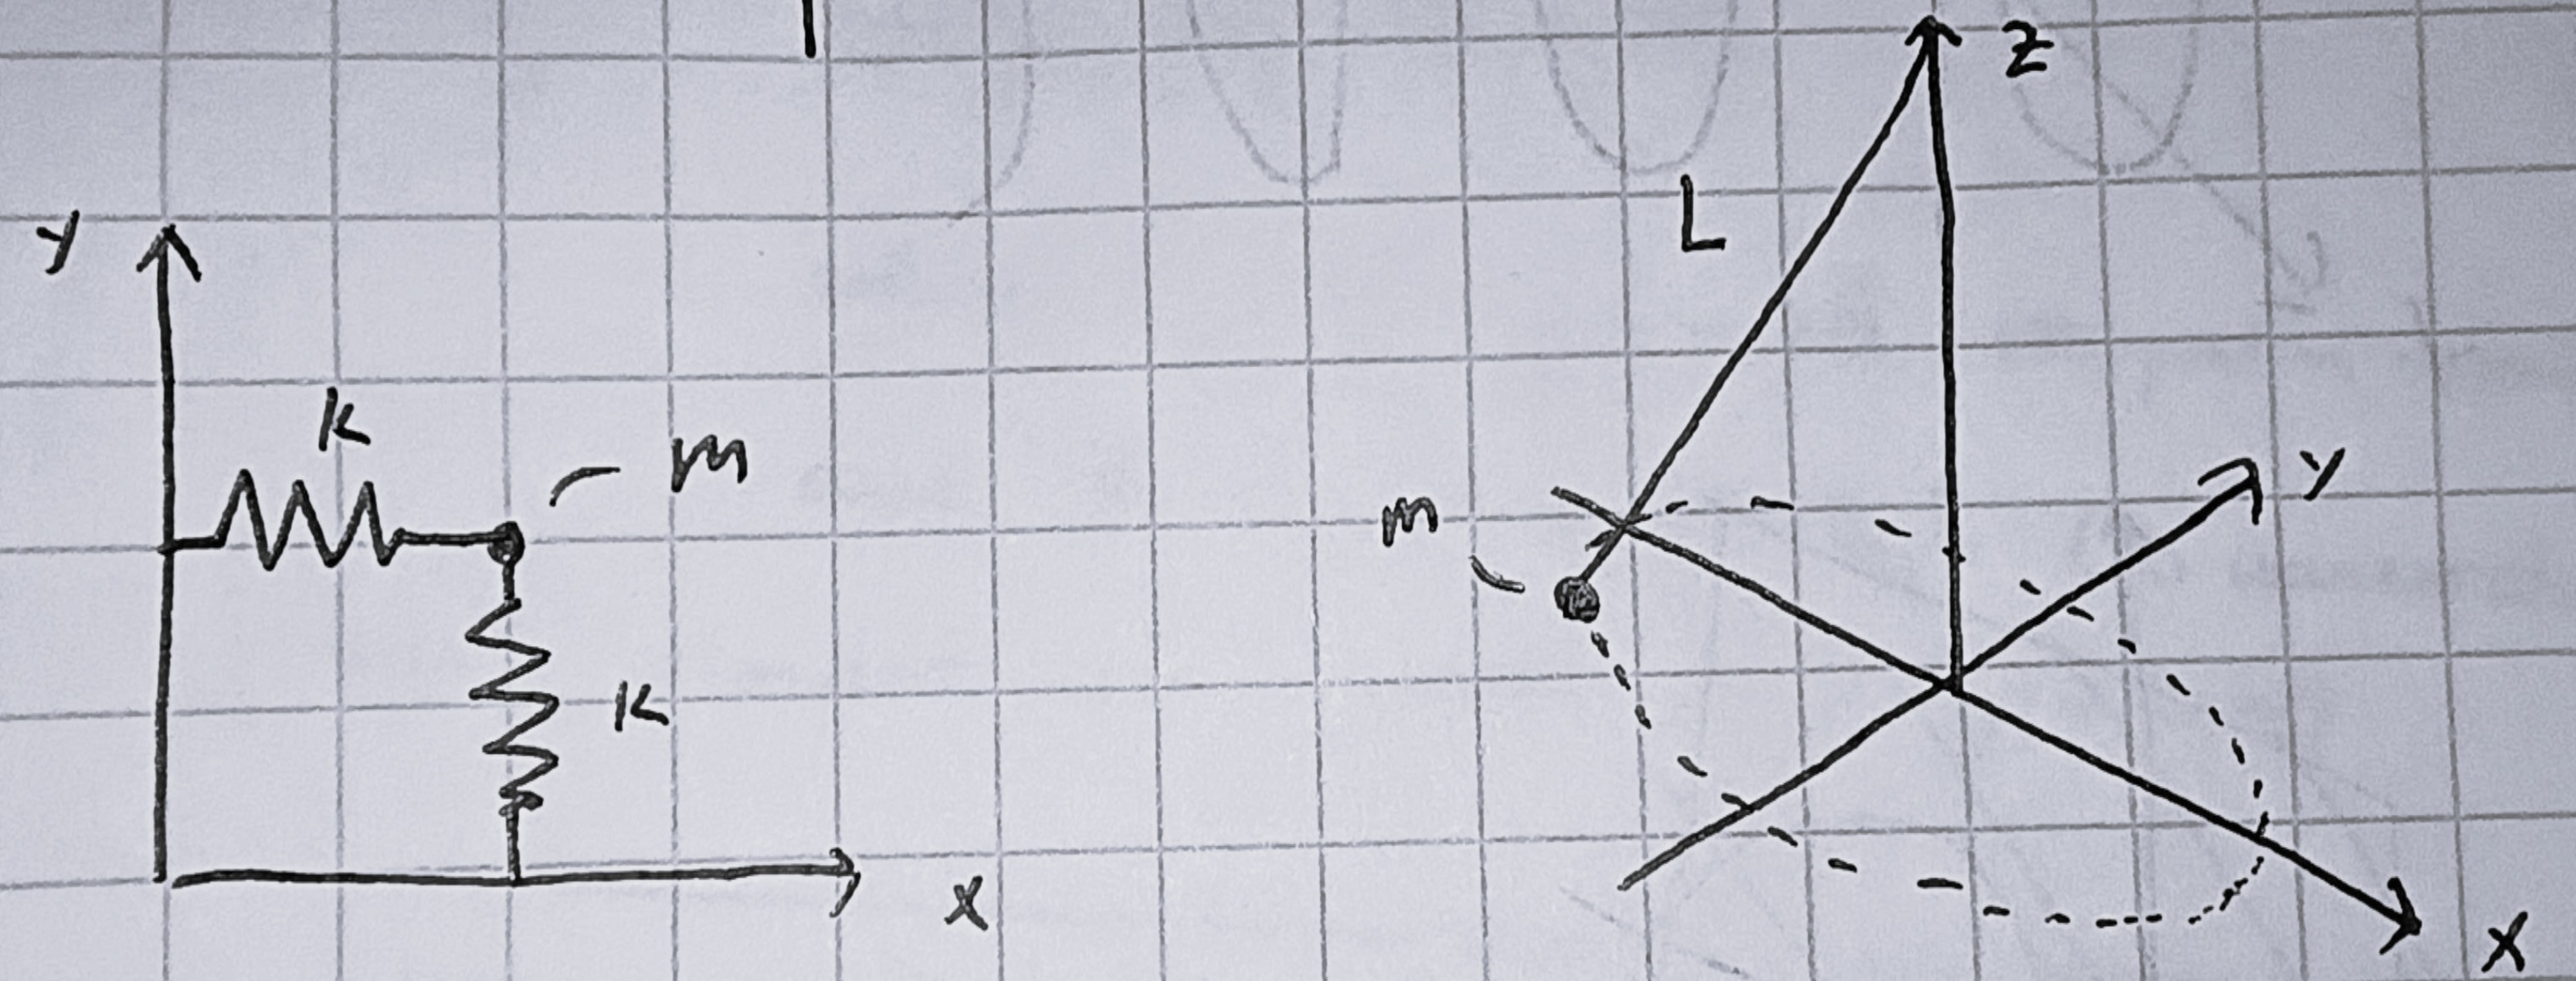
\includegraphics[width=0.8\textwidth]{SHOs.jpg}
\end{center}\newpage
\section*{General Plane Wave Solution}
We would like to generalize the case $\hat{z}$ solution
\[\vec{E} = \left( E_{0_x} e^{i \phi_x} \hat{x} + E_{0_y} e^{i \phi_y} \hat{y} \right) e^{i (k z - \omega t)}\]
to describe a plane wave propagating in an arbitrary direction. To do this, we can simply replace the $kz$ term in the phase with $\vec{k}\cdot\vec{r}$, where $\vec{k}$ is the \textbf{wavevector} that points in the direction of propagation and has magnitude $k$. This allows us to describe plane waves propagating in any direction, not just along the $z$ axis.
\[\vec{k} = k_x \hat{x} + k_y \hat{y} + k_z \hat{z}\]
\[|\vec{k}| = \sqrt{k_x^2 + k_y^2 + k_z^2} = k,\quad k= \frac{2\pi}{\lambda}\]
and $\vec{r}$ is the position vector from to origin to any point in space:
\[\vec{r} = x \hat{x} + y \hat{y} + z \hat{z}\]
Therefore, the general plane wave solution is:
\[\boxed{\vec{E} = \left( E_{0_x} e^{i \phi_x} \hat{x} + E_{0_y} e^{i \phi_y} \hat{y} \right) e^{i (\vec{k}\cdot\vec{r} - \omega t)}}\]
This general form of the plane wave solution is intuitive because it is consistent with our understanding that $\vec{E}$ depends only on spatial variations along the direction of propagation. The dot product $\vec{k}\cdot\vec{r}$ extracts the component of $\vec{r}$ in the direction of $\vec{k}$, which for case $\hat{z}$ reduces to variations along the $z$ axis. At the same time, $\vec{E}$ does not depend on spatial variations perpendicular to the direction of propagation (it is a transverse wave). For any $\vec{r}$ perpendicular to $\vec{k}$, we have $\vec{k}\cdot\vec{r}=0$, so in case $\hat{z}$ there are no variations in the $x$ and $y$ directions.\\\\
\textbf{Useful Properties of the General Plane Wave Form}\\
Time derivative
\[\frac{\partial \vec{E}}{\partial t} = -i\omega \vec{E},\quad \frac{\partial^2\vec{E}}{\partial t^2} = -\omega^2 \vec{E}\]
Spatial derivative
\[\vec{\nabla} \cdot \vec{E} = i\vec{k} \cdot \vec{E},\quad \nabla^2 \vec{E} = -k^2 \vec{E}\]
\[\vec{\nabla} \times \vec{E} = i \vec{k} \times \vec{E}\]
\underline{Note:} These properties follow from the fact that the only spatial and temporal dependence of $\vec{E}$ is contained in the phase $(\vec{k}\cdot\vec{r}-\omega t)$. When taking derivatives, the complex amplitude vector can therefore be treated as a constant, and the chain rule applies directly to the exponential term.\\\\
Also since we can find the direction of the magnetic field $\vec{B}$ using Faraday's law ($\vec{\nabla}\times\vec{E} = i\hat{k}\times\vec{E} $) and the relationship between the magnitudes of $\vec{E}$ and $\vec{B}$ ($|\vec{E}| = c|\vec{B}|$), we can also write:
\[\boxed{\vec{B}=\frac{1}{c}\hat{k}\times\vec{E}}\]
\newpage\noindent
\textbf{Constraints on Plane Wave Solutions from Maxwell's Equations}\\
For \textbf{case $\mathbf{\hat{z}}$}, we have the general plane wave solution of the form
\[\vec{E} = E_x \hat{x} + E_y \hat{y} + E_z \hat{z}\]
\[\vec{B} = B_x \hat{x} + B_y \hat{y} + B_z \hat{z}\]
Where $E_x$, $E_y$, $E_z$, $B_x$, $B_y$, and $B_z$  are complex functions of the form:
\[E_x = E_{0_x} e^{i (kz - \omega t + \phi_{x_E})}\]
Using the properties of time and spatial derivatives of the general plane wave form, we can apply Maxwell's equations to derive constraints on the components of $\vec{E}$ and $\vec{B}$.\\\\
\underline{(1) Applying Gauss's law for electricity:}
\[\vec{\nabla} \cdot \vec{E} = 0 \]
\[\left(\frac{\partial E_x}{\partial x} + \frac{\partial E_y}{\partial y} + \frac{\partial E_z}{\partial z}\right) = 0\]
Since $E_x$ and $E_y$ are only dependent on $z$ and $t$, their spatial derivatives with respect to $x$ and $y$ are zero. 
\[\frac{\partial E_x}{\partial x} = \frac{\partial E_y}{\partial y} = 0\]
Thus,
\[\frac{\partial E_z}{\partial z} = \frac{\partial}{\partial z} \left( E_{0_z} e^{i (kz - \omega t+\phi_{z_E})} \right) = 0\]
\[\implies ik E_{0_z} e^{i (kz - \omega t+\phi_{z_E})} =0\]
Since the exponential term is never zero, $\boxed{E_{0_z}\text{ must be zero}}$.\\\\
This matches our expectation that the electric field of a plane wave must be transverse to the direction of propagation, so there can be no $z$ component of the electric field for case $\hat{z}$.\\\\
\underline{(2) Applying Gauss's law for magnetism:}
\[\vec{\nabla} \cdot \vec{B} = 0\]
Similarly to (1), we can see that $B_{0_z}$ must also be zero. Also note that the lack of an $x$ and $y$ dependence in both $\vec{E}$ and $\vec{B}$ shows that the fields are \textit{uniform} across the entire $xy$ plane, which is consistent with the plane wave approximation.\\\\
\underline{(3) Applying Faraday's law:} Setting $E_{0_z}$ and $B_{0_z}$ to zero as found in (1) and (2).
\[\vec{\nabla}\times\vec{E} = -\frac{\partial \vec{B}}{\partial t}\]
\[\begin{aligned}
\begin{vmatrix} 
\hat{x} & \hat{y} & \hat{z} \\ 
\frac{\partial}{\partial x} & \frac{\partial}{\partial y} & \frac{\partial}{\partial z} \\ 
E_x & E_y & 0 
\end{vmatrix} &= -\frac{\partial}{\partial z} E_y \hat{x} + \frac{\partial}{\partial z} E_x \hat{y} + \underbrace{\left( \frac{\partial}{\partial x} E_y - \frac{\partial}{\partial y} E_x \right)}_{0} \hat{z}\\
&= -\frac{\partial}{\partial z} \left( E_{0_y} e^{i (kz - \omega t + \phi_{y_E})} \right) \hat{x} + \frac{\partial}{\partial z} \left( E_{0_x} e^{i (kz - \omega t + \phi_{x_E})} \right) \hat{y}\\
&= -ik E_{0_y} e^{i (kz - \omega t + \phi_{y_E})} \hat{x} + ik E_{0_x} e^{i (kz - \omega t + \phi_{x_E})} \hat{y}\\
&= ik e^{i (kz - \omega t)} \left( -E_{0_y} e^{i \phi_{y_E}} \hat{x} + E_{0_x} e^{i \phi_{x_E}} \hat{y} \right)
\end{aligned}\]
Now solving for $-\frac{\partial \vec{B}}{\partial t}$.
\[\begin{aligned}
    -\frac{\partial}{\partial t}\left(B_x \hat{x} + B_y \hat{y}\right) &= -\left[\frac{\partial}{\partial t}\left(B_{0_x} e^{i (kz - \omega t + \phi_{x_B})}\right)\hat{x} + \frac{\partial}{\partial t}\left(B_{0_y} e^{i (kz - \omega t + \phi_{y_B})}\right) \hat{y}\right]\\
    &= -\left[-i\omega B_{0_x} e^{i (kz - \omega t + \phi_{x_B})}\hat{x} - i\omega B_{0_y} e^{i (kz - \omega t + \phi_{y_B})} \hat{y}\right]\\
    &= i\omega e^{i (kz - \omega t)} \left(B_{0_x} e^{i \phi_{x_B}} \hat{x} + B_{0_y} e^{i \phi_{y_B}} \hat{y}\right)
\end{aligned}\]
Setting them equal to each other gives:
\[k \left( -E_{0_y} e^{i \phi_{y_E}} \hat{x} + E_{0_x} e^{i \phi_{x_E}} \hat{y} \right) = \omega \left(B_{0_x} e^{i \phi_{x_B}} \hat{x} + B_{0_y} e^{i \phi_{y_B}} \hat{y}\right)\]
Looking at the $x$ components, the magnitudes and phases must match:
\[\begin{aligned}
    -kE_{0_y}e^{i\phi_{y_E}} &= \omega B_{0_x} e^{i\phi_{x_B}} \\
    \implies E_{0_y}e^{i\pi}e^{i\phi_{y_E}} &= \frac{\omega}{k} B_{0_x}e^{i\phi_{x_B}} \\
\end{aligned}\]
Thus,
\[\boxed{\frac{E_{0_y}}{B_{0_x}} = \frac{\omega}{k} = c, \quad \phi_{y_E} + \pi= \phi_{x_B}}\]
Looking at the $y$ components, the magnitudes and phases must match:
\[\begin{aligned}
    kE_{0_x}e^{i\phi_{x_E}} &= \omega B_{0_y} e^{i\phi_{y_B}} \\
    \implies E_{0_x}e^{i\phi_{x_E}} &= \frac{\omega}{k} B_{0_y} e^{i\phi_{y_B}} \\
\end{aligned}\]
Thus,
\[\boxed{\frac{E_{0_x}}{B_{0_y}} = \frac{\omega}{k} = c, \quad \phi_{x_E} = \phi_{y_B}}\]
\underline{(4) Applying Ampere-Maxwell law:} Setting $E_{0_z}$ and $B_{0_z}$ to zero as found in (1) and (2).
\[\vec{\nabla} \times \vec{B} = \frac{1}{c^2} \frac{\partial \vec{E}}{\partial t}\]
We will see the same relationships found in (3) emerge, physics is consistent!
\[\begin{aligned}
\begin{vmatrix} 
\hat{x} & \hat{y} & \hat{z} \\ 
\frac{\partial}{\partial x} & \frac{\partial}{\partial y} & \frac{\partial}{\partial z} \\ 
B_x & B_y & 0 
\end{vmatrix} &= -\frac{\partial}{\partial z} B_y \hat{x} + \frac{\partial}{\partial z} B_x \hat{y} + \underbrace{\left( \frac{\partial}{\partial x} B_y - \frac{\partial}{\partial y} B_x \right)}_{0} \hat{z}\\
&= -\frac{\partial}{\partial z} \left( B_{0_y} e^{i(kx - \omega t + \phi_{y_B})} \right) \hat{x} + \frac{\partial}{\partial z} \left( B_{0_x} e^{i(kx - \omega t + \phi_{x_B})} \right) \hat{y}\\
&= i k e^{i(kx - \omega t)} \left[ -B_{0_y} e^{i \phi_{y_B}} \hat{x} + B_{0_x} e^{i \phi_{x_B}} \hat{y} \right]
\end{aligned}\]
Now solving for $\frac{1}{c^2} \frac{\partial \vec{E}}{\partial t}$. 
\[\begin{aligned}
\frac{1}{c^2} \frac{\partial}{\partial t} (E_x \hat{x} + E_y \hat{y}) &= \frac{1}{c^2} \left[ \frac{\partial}{\partial t} (E_{0_x} e^{i(kx - \omega t + \phi_{x_E})}) \hat{x} + \frac{\partial}{\partial t} (E_{0_y} e^{i(kx - \omega t + \phi_{y_E})}) \hat{y} \right] \\
&= \frac{1}{c^2} \left[ -i \omega E_{0_x} e^{i(kx - \omega t + \phi_{x_E})} \hat{x} - i \omega E_{0_y} e^{i(kx - \omega t + \phi_{y_E})} \hat{y} \right] \\
&= -\frac{1}{c^2} i \omega e^{i(kx - \omega t)} \left[ E_{0_x} e^{i \phi_{x_E}} \hat{x} + E_{0_y} e^{i \phi_{y_E}} \hat{y} \right]
\end{aligned}\]
$\hat{x}$ components:
\[\begin{aligned}
-k B_{0_y} e^{i \phi_{y_B}} &= -\frac{1}{c^2} \omega E_{0_x} e^{i \phi_{x_E}} \\
\implies B_{0_y} e^{i \phi_{y_B}} &= \frac{1}{c^2} \frac{\omega}{k} E_{0_x} e^{i \phi_{x_E}} \quad \implies \boxed{B_{0_y} = \frac{1}{c} E_{0_x}, \quad \phi_{y_B} = \phi_{x_E}}
\end{aligned}\]
$\hat{y}$ components:
\[\begin{aligned}
k B_{0_x} e^{i \phi_{x_B}} &= -\frac{1}{c^2} \omega E_{0_y} e^{i \phi_{y_E}} \\
\implies B_{0_x} e^{i \phi_{x_B}} &= \frac{1}{c^2} \frac{\omega}{k} E_{0_y} e^{i \pi} e^{i \phi_{y_E}} \quad \implies \boxed{B_{0_x} = \frac{1}{c} E_{0_y}, \quad \phi_{x_B} = \phi_{y_E} + \pi}
\end{aligned}\]
\underline{A \textit{slightly} better method}\\
Regrettably, while this previous method is rigorous, it is also very tedious and didn't use our newfound properties of general plane wave derivatives! Below is a (quick, I hope) method from Professor Corn:\\\\
We saw from before that when applying Faraday's law, we get
\[\vec{\nabla}\times\vec{E} = -\frac{\partial \vec{B}}{\partial t}\]
\[-\frac{\partial E_y}{\partial z}\hat{x} + \frac{\partial E_x}{\partial z}\hat{y} = -\frac{\partial B_x}{\partial t}\hat{x} - \frac{\partial B_y}{\partial t}\hat{y}\]
Setting the terms equal:
\[\implies \frac{\partial E_y}{\partial z}= \frac{\partial B_x}{\partial t} \quad \text{and} \quad \frac{\partial E_x}{\partial z}= -\frac{\partial B_y}{\partial t}\]
From the general plane wave solution:
\[\begin{aligned}
\frac{\partial E_y}{\partial z} &= \frac{\partial}{\partial z} \left[ E_{0_y} e^{i \phi_{y_E}} e^{i(kz - \omega t)} \right] = i k E_y \quad \text{and} \quad \frac{\partial E_x}{\partial z} = i k E_x \\
\frac{\partial B_x}{\partial t} &= \frac{\partial}{\partial t} \left[ B_{0_x} e^{i \phi_{x_B}} e^{i(kz - \omega t)} \right] = -i \omega B_x \quad \text{and} \quad \frac{\partial B_y}{\partial t} = -i \omega B_y
\end{aligned}\]
\[\begin{aligned}
&\implies i k E_y = -i \omega B_x && \implies i k E_x = -(-i \omega B_y) \\
&\qquad \frac{E_y}{B_x} = \frac{-\omega}{k} = -c && \qquad \frac{E_x}{B_y} = \frac{\omega}{k} = c \\
\end{aligned}\]
Plugging in for $E_x$, $E_y$, $B_x$, and $B_y$:
\[\frac{E_y}{B_x} = \frac{E_{0_y} e^{i \phi_{y_E}} e^{i(kz - \omega t)}}{B_{0_x} e^{i \phi_{x_B}} e^{i(kz - \omega t)}} = \frac{E_{0_y}}{B_{0_x}} e^{i(\phi_{y_E} - \phi_{x_B})} = -c, \quad -c = ce^{i\pi}\]
Equating the magnitudes and phases once again gives:
\[\frac{E_{0_y}}{B_{0_x}} = c \quad \text{and} \quad \phi_{y_E} - \phi_{x_B} = \pi\]
Similarly for the $x$ component:
\[\frac{E_x}{B_y} = \frac{E_{0_x} e^{i \phi_{x_E}} e^{i(kz - \omega t)}}{B_{0_y} e^{i \phi_{y_B}} e^{i(kz - \omega t)}} = \frac{E_{0_x}}{B_{0_y}} e^{i(\phi_{x_E} - \phi_{y_B})} = c\]
Equating the magnitudes and phases once again gives:
\[\frac{E_{0_x}}{B_{0_y}} = c \quad \text{and} \quad \phi_{x_E} - \phi_{y_B} = 0\]
\underline{Note}: If we didn't add in a phase difference of $\pi$ then we would see that $E_{0_y}/B_{0_x} = -\omega/k$. In either case, the right-hand rule requires $E_{0_y}$ and $B_{0_x}$ to have opposite signs since $\vec{E}\times\vec{B}$ always points in the $\vec{k}$ direction. This can be expressed either by introducing a phase difference of $\pi$ or by keeping the negative sign in the ratio.
\begin{center}
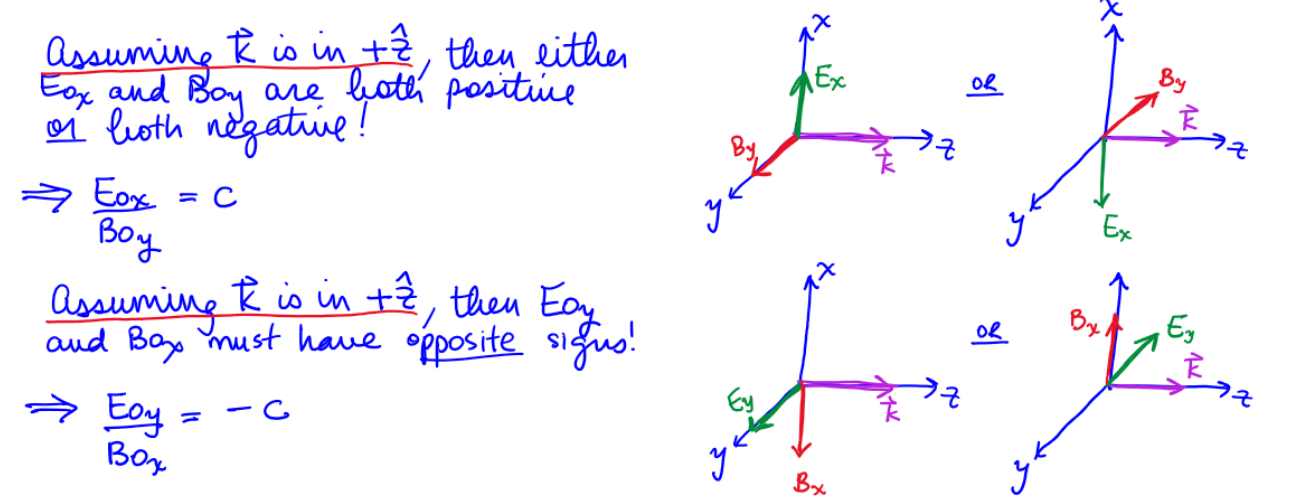
\includegraphics[width=1\textwidth]{RHR.png}
\end{center}
\section*{Energy Transported by EM Waves}
Recall that energy is stored in the electric and magnetic fields, with energy densities given by
\[u_E = \frac{1}{2} \varepsilon_0 |\vec{E}|^2 \quad (\text{energy density of electric field})\]
\[u_B = \frac{1}{2 \mu_0} |\vec{B}|^2 \quad (\text{energy density of magnetic field})\]
\underline{Note:} As mentioned before, since we are now dealing with physically measurable quantities of the $\vec{E}$ and $\vec{B}$ fields, we need to use the \textit{real} components of the fields.\\\\
Additionally, we are ignoring phase differences for now to simplify calculations, so $\phi_x = \phi_y = \phi_z = 0$ for the electric field (this simplification also applies to the magnetic field, but we'll focus on just the electric field for now).
\[\vec{E} = \Re\! \Big\{ \vec{E}_{\text{complex}} \Big\} 
= \Re\! \Big\{ \big( E_{0_x} \hat{x} + E_{0_y} \hat{y} + E_{0_z} \hat{z} \big) e^{i (\vec{k} \cdot \vec{r} - \omega t)} \Big\}\]
\[\vec{E} = 
E_{0_x} \cos(\vec{k} \cdot \vec{r} - \omega t)\,\hat{x}
+ E_{0_y} \cos(\vec{k} \cdot \vec{r} - \omega t)\,\hat{y}
+ E_{0_z} \cos(\vec{k} \cdot \vec{r} - \omega t)\,\hat{z}\]
Now the magnitude of the electric field is given by the dot product:
\[|\vec{E}|^2 = \vec{E}\cdot\vec{E} = |\vec{E}_0|^2 \cos^2(\vec{k} \cdot \vec{r} - \omega t),\quad \text{where} \quad \vec{E}_0 = E_{0_x} \hat{x} + E_{0_y} \hat{y} + E_{0_z} \hat{z}\]
\underline{For EM Waves}
\begin{itemize}
    \item Since the magnitudes of the electric and magnetic fields are related by $|\vec{E}| = c |\vec{B}|$, the energy densities of the electric and magnetic fields are also equal ($c = \frac{1}{\sqrt{\varepsilon_0 \mu_0}}$):
    \[\boxed{u_E = u_B}\]
    \item The \textbf{total energy density} $u$ is then the sum of the electric and magnetic energy densities:
    \[\boxed{u = u_E + u_B = 2u_E = \varepsilon_0 |\vec{E}|^2}\]
\end{itemize}
\textbf{Poynting Vector $\vec{S}$}
We can derive the Poynting vector $\vec{S}$, which describes the flow of electromagnetic energy carried by the $\vec{E}$ and $\vec{B}$ fields in the direction of $\vec{k}$. Its units are power per unit area, W/m$^2$. We can derive $\vec{S}$ by applying the \textit{continuity equation} (local conservation of energy) to the energy density $u$. We should expect to see that:
\[
\frac{\partial u}{\partial t} + \nabla \cdot \vec{S} = 0,
\]
Similar to how we relate the change in charge density to the divergence of current density in the continuity equation for charge, here the change in energy density is related to the divergence of the Poynting vector which describes the rate at which energy flows through an area.\\\\
Starting from $u = \frac{1}{2} \varepsilon_0 \vec{E}\cdot\vec{E} + \frac{1}{2\mu_0} \vec{B}\cdot\vec{B}$, we want to show that $\frac{\partial u}{\partial t} =- \vec{\nabla} \cdot \vec{S}$:
\[
\frac{\partial u}{\partial t} = \frac{\partial}{\partial t} \left[\frac{1}{2} \varepsilon_0 \vec{E}\cdot\vec{E} + \frac{1}{2\mu_0} \vec{B}\cdot\vec{B}\right] = \frac{1}{2} \varepsilon_0 \frac{\partial}{\partial t}(\vec{E}\cdot\vec{E}) + \frac{1}{2\mu_0} \frac{\partial}{\partial t}(\vec{B}\cdot\vec{B}) 
\]
Applying the product rule to the dot products:
\[\frac{\partial}{\partial t}(\vec{E}\cdot\vec{E}) = 2\vec{E}\cdot\frac{\partial \vec{E}}{\partial t} \quad \text{and} \quad \frac{\partial}{\partial t}(\vec{B}\cdot\vec{B}) = 2\vec{B}\cdot\frac{\partial \vec{B}}{\partial t}\]
\[\implies \frac{\partial u}{\partial t} = \varepsilon_0 \vec{E}\cdot\frac{\partial \vec{E}}{\partial t} + \frac{1}{\mu_0} \vec{B}\cdot\frac{\partial \vec{B}}{\partial t}\]
From Faraday's Law:
\[\vec{\nabla} \times \vec{E} = -\frac{\partial \vec{B}}{\partial t} \quad\implies\quad \frac{\partial \vec{B}}{\partial t} = -\vec{\nabla} \times \vec{E}\]
From Ampere-Maxwell Law:
\[\vec{\nabla} \times \vec{B} = \mu_0 \varepsilon_0 \frac{\partial \vec{E}}{\partial t} \quad\implies\quad \frac{\partial \vec{E}}{\partial t} = \frac{1}{\mu_0 \varepsilon_0} \vec{\nabla} \times \vec{B}\]
Substituting these into the expression for $\frac{\partial u}{\partial t}$:
\[\begin{aligned}
\frac{\partial u}{\partial t} &= \varepsilon_0 \vec{E}\cdot\left(\frac{1}{\mu_0 \varepsilon_0} \vec{\nabla} \times \vec{B}\right) + \frac{1}{\mu_0} \vec{B}\cdot(-\vec{\nabla} \times \vec{E})\\
&= \frac{1}{\mu_0} \left[\vec{E}\cdot(\vec{\nabla} \times \vec{B}) - \vec{B}\cdot(\vec{\nabla} \times \vec{E})\right]\\
&= \frac{1}{\mu_0} \left[-\vec{\nabla} \cdot (\vec{E} \times \vec{B})\right]
\end{aligned}\]
\underline{Note:} The last step uses the vector identity $\vec{\nabla} \cdot (\vec{A} \times \vec{B}) = \vec{B}\cdot(\vec{\nabla} \times \vec{A}) - \vec{A}\cdot(\vec{\nabla} \times \vec{B})$.\\\\
Therefore, the Poynting vector is
\[\boxed{\vec{S} = \frac{1}{\mu_0} \vec{E} \times \vec{B}}\]
It is also equivalent to 
\[\vec{S} = \frac{1}{\mu_0} \vec{E}\times\vec{B} = \frac{1}{\mu_0} |\vec{E}|\underbrace{|\vec{B}|}_{\frac{1}{c}|\vec{E}|}\hat{k} = \underbrace{\frac{1}{\mu_0 c}}_{\varepsilon_0 c} |\vec{E}|^2 \hat{k}\]
\[\implies \boxed{\vec{S} = cu\hat{k}}\]
\textbf{Intensity}\\
Intensity is defined as the time-averaged magnitude of the Poynting vector, which describes the \textit{average} power per unit area carried by the electromagnetic wave.
\[\langle\vec{S}\rangle = c \langle u \rangle, \qquad \langle\quad\rangle: \text{ time average}\]
Where
\[\langle u \rangle = \varepsilon_0 \langle |\vec{E}|^2 \rangle = \varepsilon_0 E_0^2 \langle \cos^2(\vec{k} \cdot \vec{r} - \omega t) \rangle = \frac{1}{2} \varepsilon_0 E_0^2\]
The time average of $\cos^2$ is 1/2 because the function oscillates between 0 and 1, and over a full period, it spends equal time at all values in that range. Therefore, the average value of $\cos^2$ over one period is 1/2.\\\\
Thus, the intensity of an electromagnetic wave is given by
\[\boxed{I = \langle\vec{S}\rangle = c \langle u \rangle=\frac{1}{2} \varepsilon_0 E_0^2 c}\]
\underline{Note:} A higher light intensity corresponds to a larger electric-field amplitude, meaning the wave transports energy at a greater rate per unit area. This aligns with the physical interpretation of intensity as a measure of brightness: brighter light delivers more energy to a surface per unit time.
\vspace{1em}
\noindent\hrule
\vspace{1em}
\newpage
\begin{center}
   {\LARGE Unit 2: Radiation and Scattering\par} 
\end{center}
The goal of this unit is to model how electromagnetic waves are generated by an accelerated charge (via radiation and scattering) using \textit{classical physics}. Along the way, we will make some approximations and assumptions that will yield a usable model but also introduce some limitations that we will later address with quantum mechanics.
\section*{Thompson Radiation}
In the Thompson model, we are considering the electromagnetic radiation emitted by a \textit{free} charged particle previously travelling at a constant velocity (or at rest) that is accelerated by a short \textit{constant} acceleration, a "kick". This acceleration causes a kink in the electric field lines of the charge, which then propagates outward as an electromagnetic wave.\\\\
Before we begin, it is important to note the \textit{scale} of the set-up we are working with. Perhaps the most important simplifying approximation we make is that the duration of the acceleration $\tau$ is very short compared to the time \textit{after the acceleration} at which we observe the electric field, $T$ ($\tau \ll T$). Additionally, $\tau$ is so short that the final constant velocity of the charge after the acceleration remains much less than the speed of light ($v \ll c$), so we can ignore relativistic effects. Importantly, this approximation lets us treat the electric field of a charge moving at constant velocity as essentially the same as that of a static charge, except that the field now points away from the \textit{instantaneous position} of the charge rather than from a fixed point such as the origin.\\\\
For a charge moving relativistic velocity, something similar to length contraction occurs, where the electric field lines become squished along the direction of motion, and the field becomes stronger in the plane perpendicular to the motion and the lorentz factor $\gamma$ appears. For our case, $v \ll c$, so $\gamma \approx 1$ and we can ignore these relativistic effects.
\begin{center}
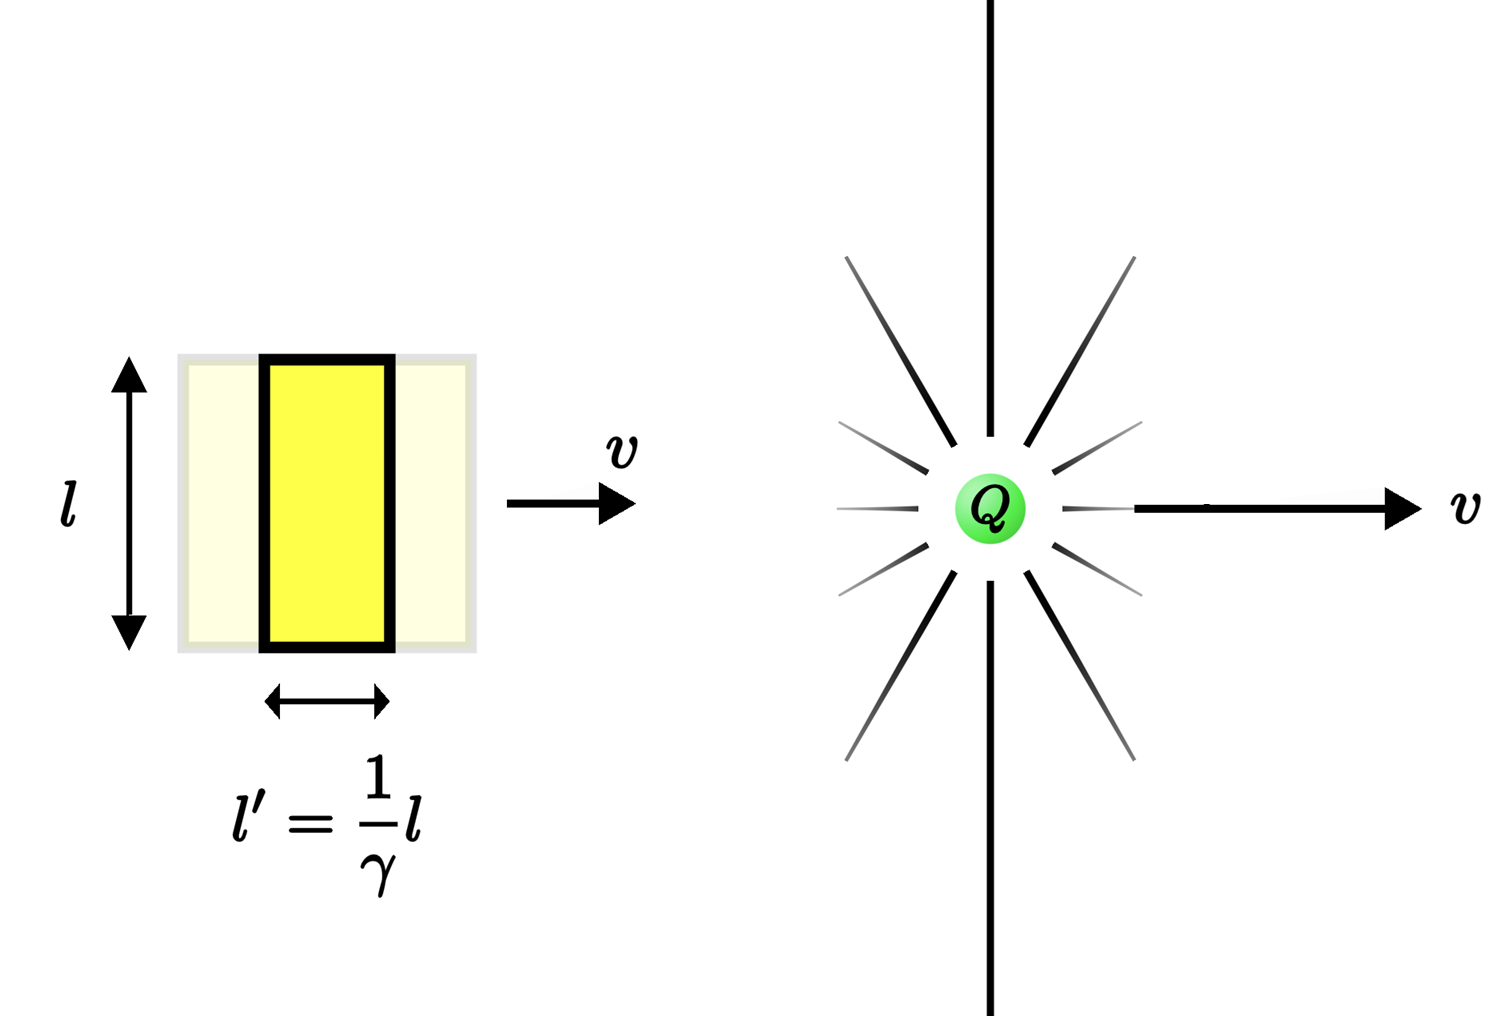
\includegraphics[width=0.6\textwidth]{E Moving Charge.png}
\end{center}
\newpage\noindent
\textbf{The Setup}
\begin{enumerate}
    \item A free charge is at rest at $x=0$ for all time $t\leq0$.
    \item The charge is "kicked" and accelerated with a constant $a$ for a short period of time $\tau$ in the $+x$ direction.
    \item After the acceleration, the charge moves at a constant velocity $v = a\tau$ in the $+x$ direction forever ($t > \tau$).
    \item We will observe the electric field lines far away from the charge and at a much later time $T$ after the acceleration ($\tau \ll T$).
\end{enumerate}
\begin{center}
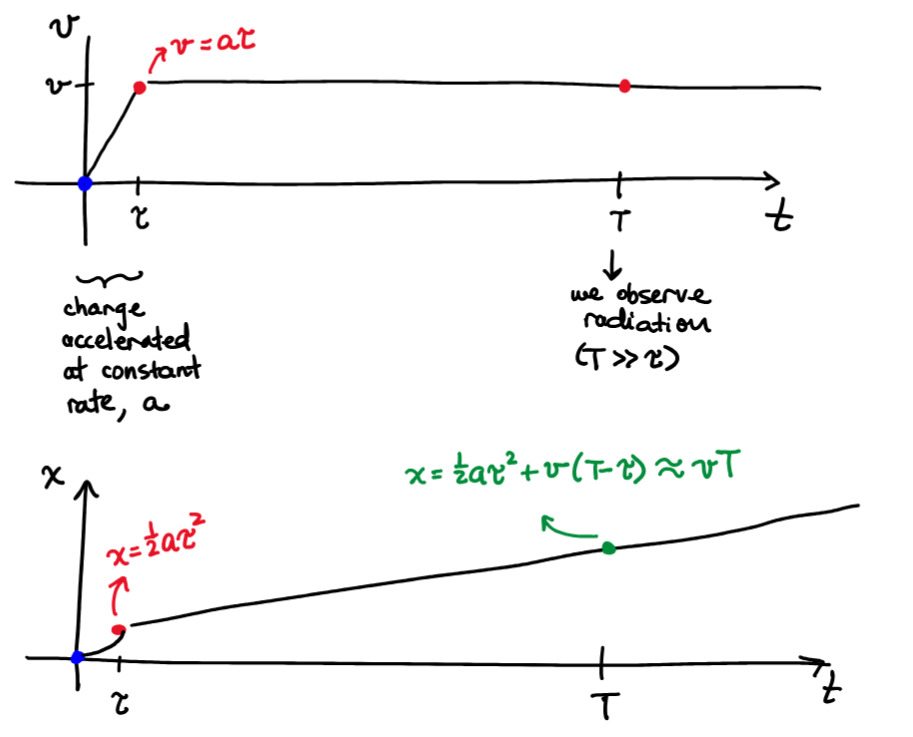
\includegraphics[width=0.8\linewidth]{Thompson Model.png}
\end{center}
\newpage\noindent
\textbf{Relativistic Causality}\\
Relativistic causality states that no information can propagate faster than the speed of light. In this model, the information of interest is the beginning and end of the acceleration of the charge. These disturbances propagate outward at speed $c$.\\\\
The outer boundary, which represents the beginning of the acceleration, is a sphere of radius centered at the origin, corresponding to the physical position of the charge at $t = 0$.
\[R_0 = cT\]
Likewise, the inner boundary, which represents the end of the acceleration, is a sphere of radius centered at $x = \frac{1}{2} a \tau^2$ which is the physical position of the charge at $t = \tau$.
\[R_1 = c(T - \tau)\]
\begin{center}
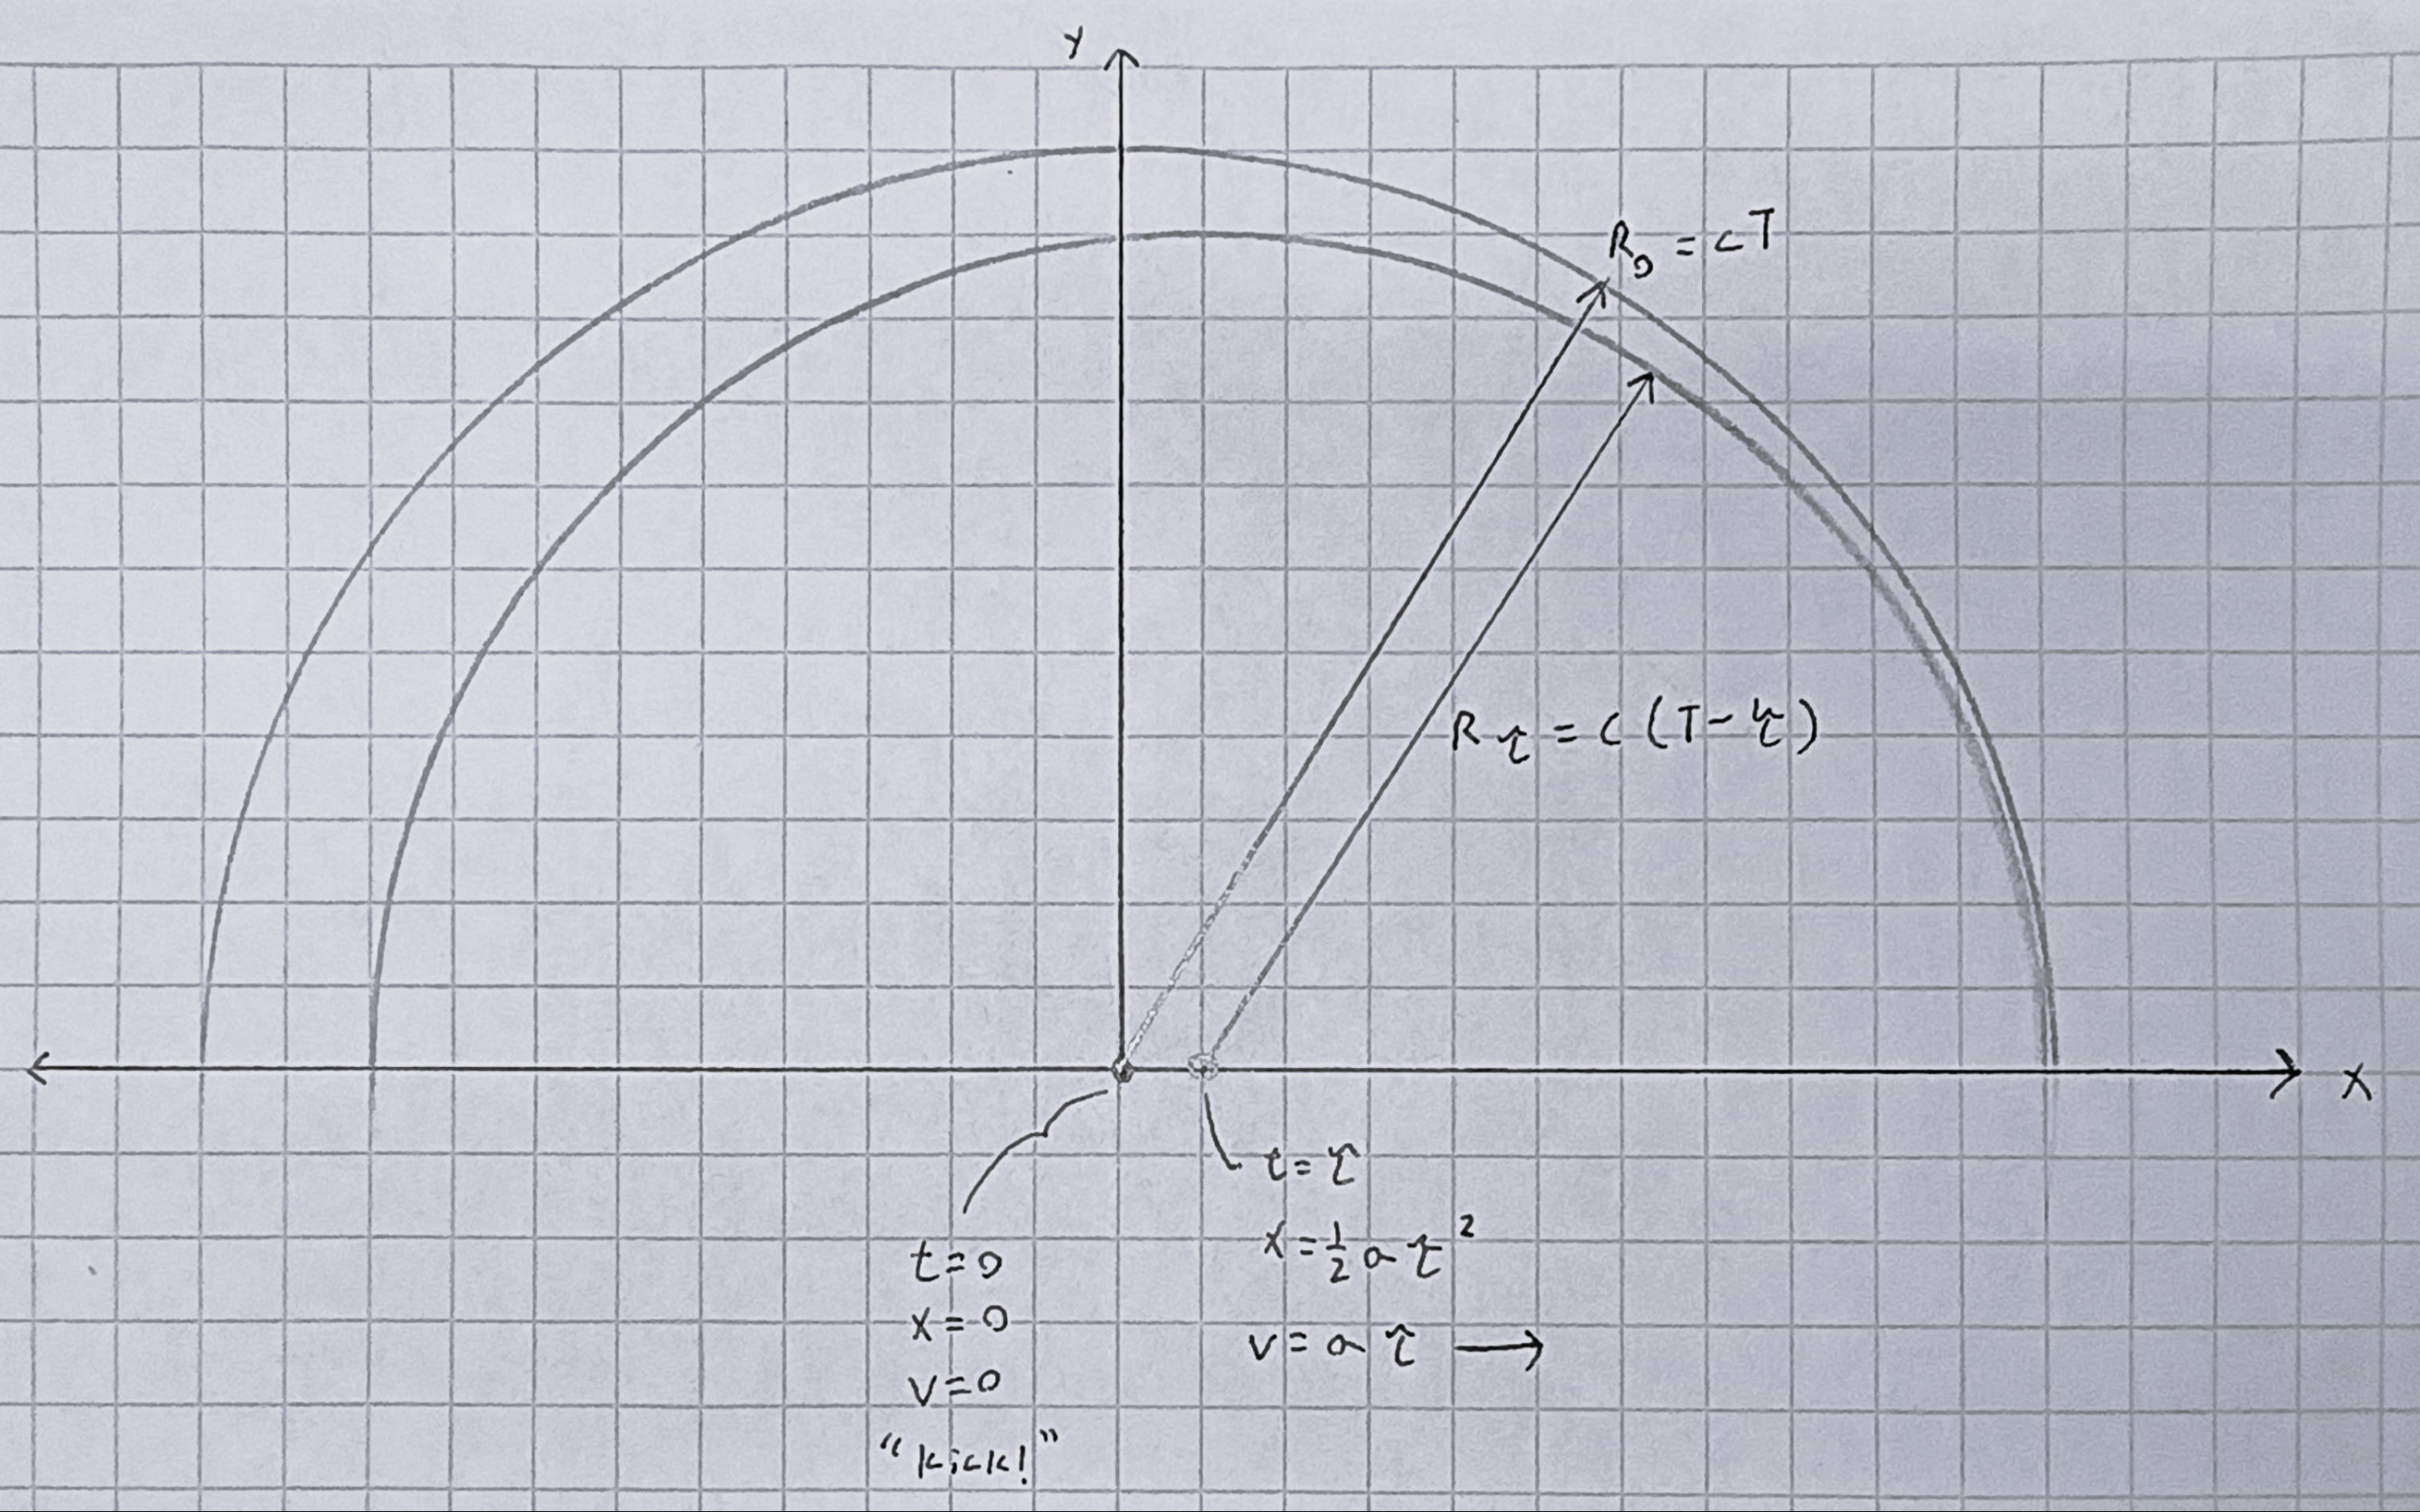
\includegraphics[width=1\linewidth]{Thompson Model-1.jpg}
\end{center}
The region between these two radii contains the kink in the electric field, that is, the electromagnetic wave. This is why we say that an accelerated charge produces radiation.\\\\
Under the approximation $\tau \ll T$ and in the limit $\tau \to 0$, the displacement of the charge during the acceleration becomes negligible. Thus, the charge's position after the acceleration is approximately the same as its initial position, and the two spheres may be treated as approximately concentric. Additionally, following our previous approximation that the electric field of a charge moving at constant velocity is essentially the same as that of a static charge, we can say that the field lines entering and exiting this region are parallel, forming the same angles to the $x$ axis. 
\begin{center}

\includegraphics[width=1\linewidth]{Thompson Model-2.jpg}
\end{center}
Due to relativistic causality, the electric field lines in region I must be that of a static charge at the origin (because the information of the acceleration has not yet reached this region). The electric field lines in region II, then, must be that of a charge moving at constant velocity (because the information of the acceleration has already reached this region).\\\\
\textbf{The Radiated Electric Field}\\
So what must the electric field be in the region in between, the spherical shell of thickness $c\tau$, which is the \textit{only} region containing information about the charge \textit{during its acceleration}? Since the electric field is continuous, the field lines must connect smoothly across this region. As a result, they develop a kink within the shell, giving the field both a radial component $E_r$ and a transverse component $E_\theta$.\\\\
We can derive the magnitudes of these components by using the geometry to decompose the electric field:\\
\begin{minipage}{0.5\textwidth}
\[\vec{E}_a = E_r \hat{r} + E_{\theta}\hat{\theta}\]
\[tan\phi = \frac{E_{\theta}}{E_r} \implies E_\theta = E_r \frac{vT\sin\theta}{c\tau}\]
Using Gauss's law, we can find $E_r$:
\[E_r = \frac{q}{4\pi\epsilon_0 R_0^2} = \frac{q}{4\pi\epsilon_0 (cT)^2}\]
Thus,
\[E_{\theta} = \frac{v}{\tau}\frac{q\sin\theta}{4\pi\varepsilon_0 c^3 T}\]
\end{minipage}
\hfill
\begin{minipage}{0.4\textwidth}
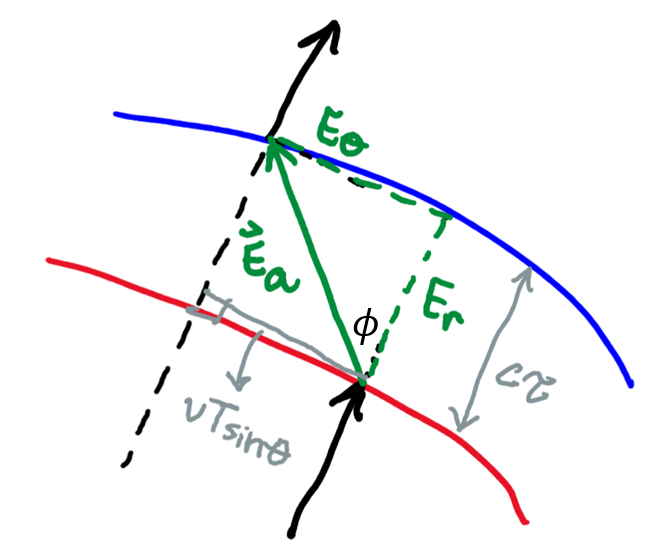
\includegraphics[width=\linewidth]{Radiated.png}
\end{minipage}
\underline{Note:} We can choose any Gaussian surface that encloses the charge. Since the electric field line is continuous, its magnitude remains the same along its entire path. However, choosing a sphere that lies entirely within region I is most convenient, because the electric flux there comes solely from the static charge at the origin due to relativistic causality. In region II, by contrast, the charge has moved and is no longer centered within the sphere, leading to a non-uniform electric flux distribution.\\\\
A more useful form for $E_\theta$ can be obtained by substituting $a = v/\tau$ and $R = cT$:
\[E_\theta = \frac{1}{4\pi\varepsilon_0} \frac{qa\sin\theta}{c^2R}\]
Therefore, the electric field kink is
\[\vec{E}_a = \frac{1}{4\pi\epsilon_0}\frac{q}{ R^2} \hat{r} + \frac{1}{4\pi\varepsilon_0} \frac{qa\sin\theta}{c^2R} \hat{\theta}\]
Since the radial component $E_r$ falls off as $1/R^2$ while the transverse component $E_\theta$ falls off as $1/R$, for large observation distances $R$, $E_r \ll E_\theta$ and the electric field is dominated by the transverse component. Therefore, for radiation, and also for quantifying the resulting electromagnetic wave, we can use just $E_\theta$, the transverse component of the electric field.\\\\
This also makes intuitive sense in our model. Since $R = cT$, a large $R$ corresponds to a large $T$, so the approximation $\tau \ll T$ becomes increasingly valid. In this limit, the region between regions I and II effectively shrinks to a spherical shell of negligible thickness, and the field lines become squished so that they are essentially tangential to the sphere, meaning they are purely transverse.\\\\
Finally, putting all the intuition and math together, we have the formula for the \textbf{Thompson radiation} generated from an accelerating charge:
\[\boxed{\vec{E}(\vec{r},t) = \frac{1}{4\pi\varepsilon_0} \frac{qa\sin\theta}{c^2|\vec{r}|}\,\hat{\theta}\quad (\text{Thompson radiation})}\]
Where:
\begin{itemize}
    \item $a$ is the acceleration of the charge.
    \item $q$ is the charge of the particle.
    \item $\theta$ is the angle between the direction of acceleration and the direction of observation.
    \item $c$ is the speed of light.
\end{itemize}
$\vec{r}$ is the position vector from the charge's initial position to the observation point, and is also the \textit{direction of the electromagnetic wave propagation $\vec{k}$}. This is because the kink in the electric field lines spreads out radially outward, while the electric field itself is always tangential to $\hat{r}$.\\\\
Also, while time $t$ doesn't explicitly appear in the formula physically, recall that the radius $|\vec{r}|$ is related to the time of observation $T$ by $|\vec{r}|=cT$. Additionally, the acceleration $a$ can also be a function of time, and the formula for Thompson radiation can be applied to each instantaneous value of $a$.\\\\
As a concluding thought, electromagnetic waves are generated by an accelerated charge fundamentally because of relativistic causality. The discrepancy between the travelling spheres of information about the beginning and the end of the acceleration simply can only be resolved by the electric field lines developing a kink in the region between the two spheres. From the arguments developed in the past four pages, this kink is not optional but required, and it is precisely this feature that constitutes the radiation field.\\\\
\begin{minipage}{0.7\textwidth}
    \vspace{-9em}
\underline{Note:} Recall from the general plane wave solution that we can also define the magnetic field \textit{induced} by the radiated electric field kink using
\[\vec{B}(\vec{r},t) = \frac{1}{c}\hat{k}\times\vec{E},\quad \hat{k}=\hat{r}\]
\end{minipage}
\hfill
\begin{minipage}{0.3\textwidth}
    \begin{center}
       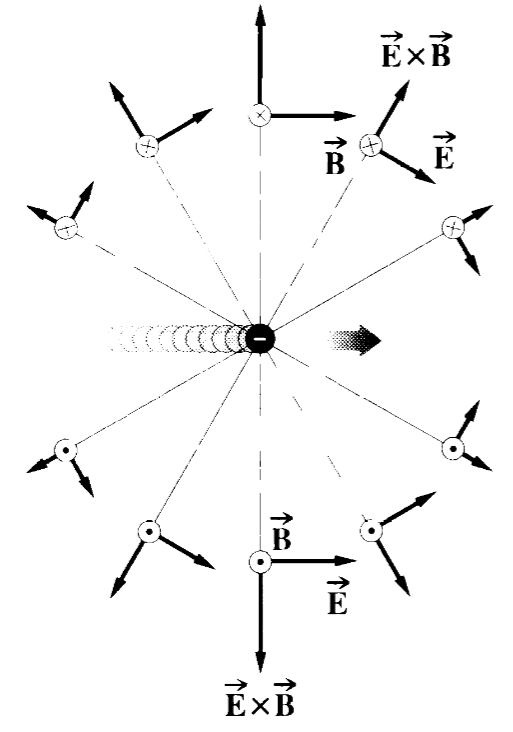
\includegraphics[width=\linewidth]{Cross-section.png} 
    \end{center}
\end{minipage}\\\\
\textbf{Poynting Flux}\\
Using the Poynting flux vector, we can calculate the rate of energy radiated by the accelerating charge:
\[\vec{S}(\vec{r},t)=\frac{1}{\mu_0}\vec{E}\times\vec{B}\]
\[\boxed{|\vec{S}|=\varepsilon_0 c |\vec{E}|^2 = \frac{q^2a^2\sin^2\theta}{16\pi^2\varepsilon_0r^2c^3}\quad\left[\frac{\text{W}}{\text{m}^2}\right]}\]
this is the power per unit area at a distance $r=|\vec{r}|$ from the charge and an angle $\theta$ from the direction of acceleration due to a short acceleration $a$.
\newpage\noindent
\textbf{What Does it Look Like?}\\
The Poynting vector \(\vec{S}\) points in the direction of electromagnetic wave propagation \(\hat{r}\), so energy flows radially outward from the charge. Thus, the radiated power spreads away from the source in spherical wavefronts, like sound waves or ripples on a pond from an isotropic source.
\begin{center}
    
\includegraphics[width=0.5\linewidth]{Ripples.png}
\end{center}
\begin{minipage}{0.5\textwidth}
    \vspace{-4em}
Power depends on the angle \(\theta\), meaning that it is strongest at \(\theta = \pi/2\) (perpendicular to the direction of acceleration) and weakest at \(\theta = 0\) or \(\pi\) (along the direction of acceleration). This results in a doughnut (toroidal) radiation pattern, with the charge at the center and the hole of the doughnut along the axis of acceleration.
\end{minipage}
\hfill
\begin{minipage}{0.4\textwidth}
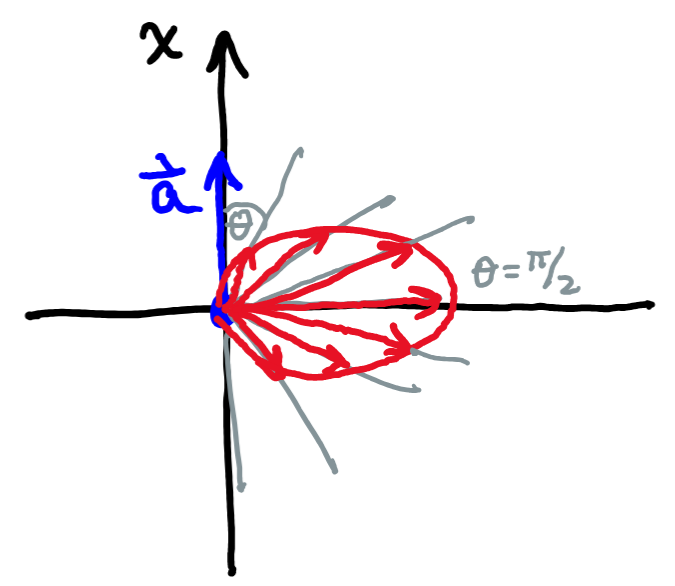
\includegraphics[width=\linewidth]{Dipole-Antenna.png}
\end{minipage}
\begin{minipage}{0.49\textwidth}
\centering
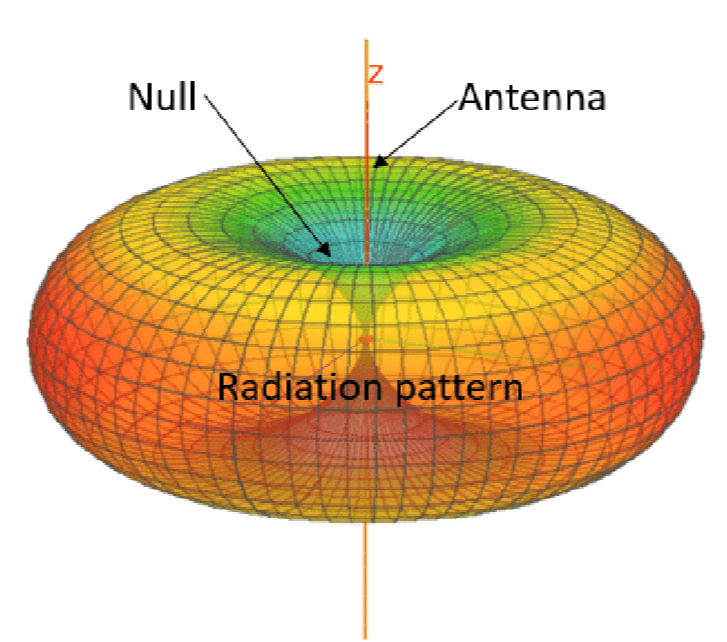
\includegraphics[width=\linewidth]{Radiation pattern.png}
\end{minipage}
\hfill
\begin{minipage}{0.49\textwidth}
\centering
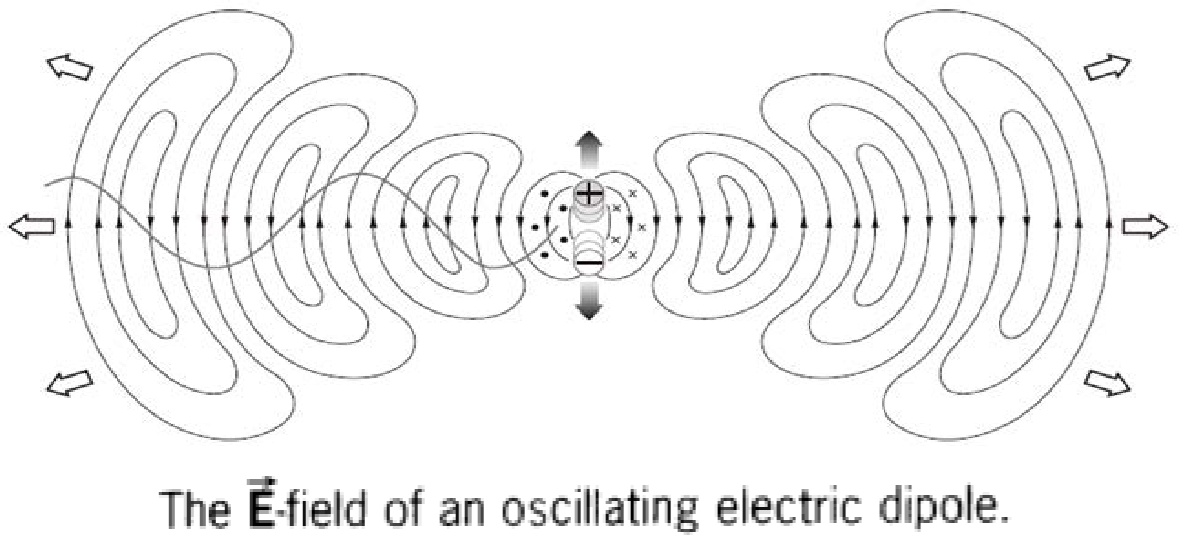
\includegraphics[width=\linewidth]{Oscilating dipole.png}
\end{minipage}
\newpage
\section*{Larmor Power}


\end{document}